\documentclass[a4paper, 12pt, french]{article}
%\immediate\write18{texcount -tex -sum -char \rapport.tex > /tmp/wordcount.tex}
\usepackage[utf8]{inputenc}
\usepackage[T1]{fontenc}
\usepackage{babel}
\usepackage{setspace}
\usepackage{hyperref}
\usepackage{imakeidx}
\usepackage{graphicx}
\usepackage{fancyhdr}
\usepackage{chngcntr}
\usepackage{pifont}
\usepackage{xcolor}
\usepackage{glossaries}
\usepackage{helvet}
\usepackage{titlesec}
\usepackage{tikz}
\usepackage{rotating}
\usepackage{lscape}
\usepackage{wrapfig}
\usepackage[stable]{footmisc}
\usepackage{comment}
\usepackage{enumitem}
\usepackage[stable]{footmisc}

\makeindex[intoc]
 
\counterwithin{figure}{section}
\counterwithin{table}{section}

\setcounter{tocdepth}{4}
\setcounter{secnumdepth}{4}
\setcounter{tocdepth}{5}
\setcounter{secnumdepth}{5}

\definecolor{ssiYellow}{RGB}{255,237,0}
\definecolor{ssiRed}{RGB}{231,0,14}
\definecolor{ssiBlack}{RGB}{18,18,13}

\newcommand{\bdot}{\item[\color{ssiYellow}\ding{108}]} 
\newcommand{\bdotoutlined}{\item[\color{ssiYellow}\ding{109}]}
\newcommand{\bsquare}{\item[\color{ssiYellow}\ding{110}]}
\newcommand{\bsquareoutlined}{\item[\color{ssiYellow}\ding{111}]}
\newcommand{\bdiamond}{\item[\color{ssiYellow}\ding{117}]}
\setlistdepth{9}
\renewlist{itemize}{itemize}{9}

%remove red border on links in the table of contents and green border for bibliography ..
%change links style : remove border by making it white
\hypersetup{%
    pdfborder = {0 0 0}
}
\renewcommand{\familydefault}{\sfdefault}

\titleformat{name=\section}{\normalfont\Large\bfseries\color{ssiBlack}}{\color{ssiYellow}\rule[-1.35mm]{3em}{1.25em}{\color{white}\hspace{-1cm}\normalfont\Large\bfseries\thesection\hspace{15pt}}}{1em}{}[\color{ssiYellow}{\titlerule[4pt]}\vspace*{4pt}]
\titleformat{\subsection}{\normalfont\Large\bfseries\color{ssiBlack}}{\color{ssiRed}\rule[-1.35mm]{3em}{1.25em}{\color{white}\hspace{-1.3cm}\normalfont\Large\bfseries\thesubsection\hspace{10pt}}}{1em}{}[\color{ssiYellow}{\titlerule[3pt]}\vspace*{4pt}]
\titleformat{\subsubsection}{\normalfont\Large\bfseries\color{ssiBlack}}{\color{ssiYellow}\rule[-1.35mm]{3em}{1.25em}{\color{white}\hspace{-1.60cm}\normalfont\Large\bfseries\thesubsubsection\hspace{5pt}}}{1em}{}[\color{ssiYellow}{\titlerule[2pt]}\vspace*{4pt}]

\titleformat{name=\section,numberless=true}{\color{ssiBlack}\normalfont\Large\bfseries}{}{0em}{}[\color{ssiYellow}{\titlerule[4pt]}\vspace*{4pt}]
\titleformat{name=\subsection,numberless=true}{\color{ssiBlack}\normalfont\Large\bfseries}{}{0em}{}[\color{ssiYellow}{\titlerule[3pt]}\vspace*{4pt}]
\titleformat{name=\subsubsection,numberless=true}{\color{ssiBlack}\normalfont\Large\bfseries}{}{0em}{}[\color{ssiYellow}{\titlerule[2pt]}\vspace*{4pt}]

\sloppy

\pagestyle{fancy}
\fancyhf{}
\rhead{Informatique et réseaux}
\lhead{PINEAU Anthony}

\makeglossaries

%\newglossaryentry{latex}{name=latex,description={Is a mark up language specially suited for scientific documents}}
%\newglossaryentry{maths}{name=mathematics,description={Mathematics is what mathematicians do}}
%\newglossaryentry{formula}{name=formula,description={A mathematical expression}}
%\newacronym{gcd}{GCD}{Greatest Common Divisor}
%\newacronym{lcm}{LCM}{Least Common Multiple}

\newglossaryentry{WMS}{name=Warehouse Management System,description={ou Système de Gestion d’Entrepôt est un logiciel informatique dédié à l’optimisation de la gestion des stocks au sein des entrepôts.\footnote{\cite{wms}}}}

\newglossaryentry{WCS}{name=Warehouse Control System,description={ou Système de Pilotage des Activités représente un outil d’optimisation du flux logistique. Un système ou logiciel WCS pilote et synchronise les différents des éléments mécanisés ( Robots, pautomates, convoyeurs, dépose étiquettes , balances ….) de l’entrepôt.\footnote{\cite{wcs}}}}

\newacronym{wms}{WMS}{Warehouse Management System}
\newacronym{wcs}{WCS}{Warehouse Control System}

\begin{document}	
	\begin{titlepage}
		\begin{center}
			\tikz[remember picture,overlay] \node[opacity=0.3,inner sep=0pt] at (current page.center){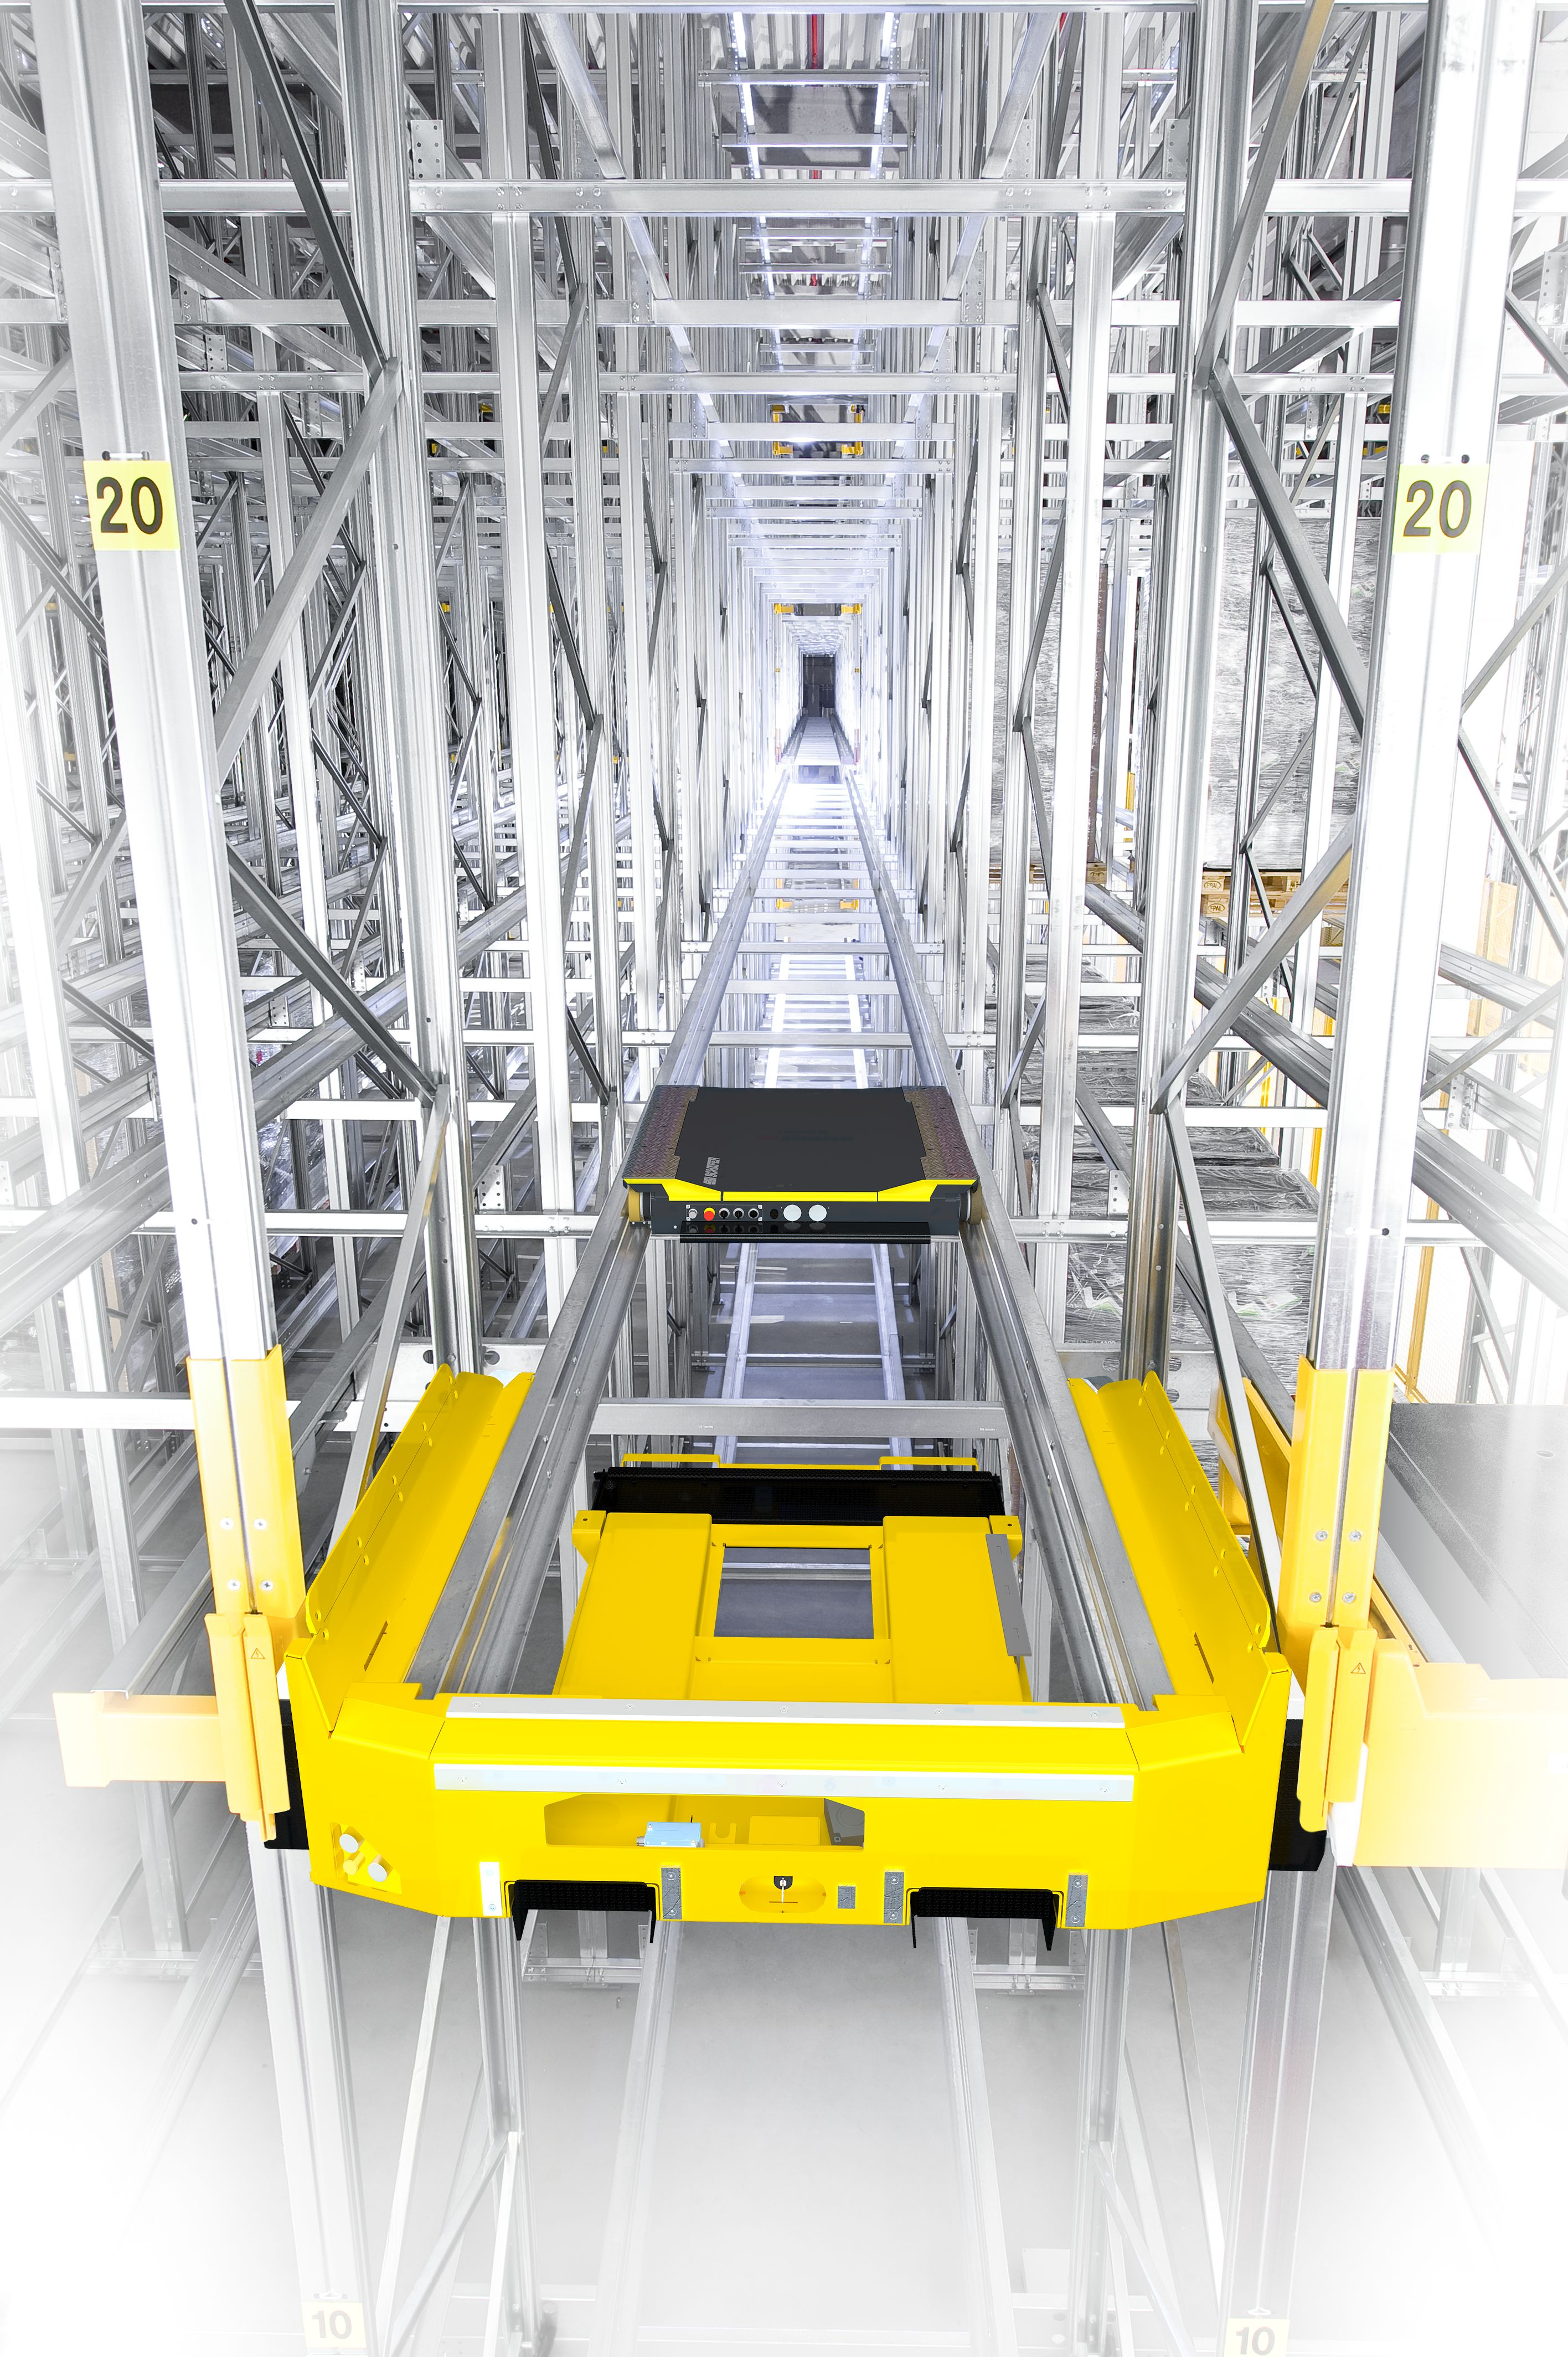
\includegraphics[width=\paperwidth,height=\paperheight]{images/ssi_orbiter_highlight.jpg}};

			\Huge
			\textbf{Mémoire de fin d'études}

			\vspace{0.5cm}
			\LARGE
			"Passer d'une application client lourd à une application web : exemple de transition d'un logiciel logistique"

			\vspace{1.5cm}

			\textbf{Anthony PINEAU}\\
			\textbf{IR2023}

			\vfill

			
\includegraphics[width=0.6\textwidth]{images/schaefer.jpg}
			\vfill
			
\includegraphics[width=0.4\textwidth]{images/esaip.jpg}

			\vfill

			Stage effectué du\\
			13 mars 2023 au 22 septembre 2023

			\vspace{0.8cm}
			
			\Large
			Maître de stage : Monsieur Thierry NEROT\\
			Tuteur pédagogique : Docteur Sofiane HAMRIOUI\\
		\end{center}
	\end{titlepage}
		
	\newpage

	\footnotesize
	\section*{Remerciements}		
		En premier lieu, je tiens à remercier Monsieur Laurent GOURDON, directeur général France de l'entreprise SSI SCHÄFER, de m’avoir permis de rejoindre à nouveau son équipe et m’avoir offert la possibilité de mettre en pratique mes connaissances et mes compétences acquises pendant mes précédentes années d’études ainsi que ces trois années du cycle ingénieur du numérique à l’ESAIP. \\

		Je tiens ensuite à remercier Monsieur Thierry NEROT, qui, en tant que maître de stage, s'est rendu disponible pour moi, et a su m'accompagner et partager ses connaissances avec moi. Il a aussi participé à la rédaction de ce mémoire en m'aidant dans la relecture et en me donnant ses conseils les plus précieux\\
-
		J’en profite pour remercier aussi tous les membres de l’équipe avec qui j’ai pu travailler, Messieurs Sébastien NICOD, Thibaut LUCAS et Pascal MARCELOT, qui ont su se rendre disponible pour moi si besoin. Il a d'ailleurs été très facile pour moi de pouvoir échanger avec eux et j'ai beaucoup appris auprès d'eux.\\

		Par ailleurs, je remercie également tous mes autres collègues qui ont été très accueillants tout au long du stage, Mesdames Charlotte BARGMAN, Océane SACHOT, Pauline CHAPRON, Anita BABONNEAU, Nathalie DELARUE, Roukia ATHOUMANI ainsi que Messieurs Quentin VIOLLEAU, Robin BALLON et Nicolas PERDRIAU.\\

		Je saisis cette occasion pour adresser mes profonds remerciements aux responsables et au personnel de l’ESAIP d’avoir fait le nécessaire en ce qui concerne la gestion des conventions de stage ainsi que de nous soutenir au quotidien dans notre projet pédagogique et professionnel.\\

		Je tiens ainsi à remercier tout particulièrement Monsieur Sofiane HAMRIOUI. En tant que tuteur pédagogique, nous avons pu échanger tout au long de mon stage, parler de l’avancement du projet sur lequel j'ai travaillé ainsi que travailler sur les parties de ce présent mémoire.\\

		Ensuite je tiens à adresser un grand merci à ma famille, sans qui tout cela ne serait pas possible. Merci pour leurs conseils ainsi que leur soutien inconditionnel, à la fois moral et économique. Ils m’accompagnent et me soutiennent au quotidien aussi bien dans mon projet pédagogique que dans mon projet professionnel et sont une source d’inspiration pour moi.\\

		Enfin je tiens à adresser un profond remerciement à ma compagne, Madame Antonia HAMMER, pour son soutien tout au long de mon stage, pour son aide pour la rédaction des parties en allemand de ce présent mémoire ainsi que pour la préparation de la partie allemande de la soutenance. Vielen Dank meine Liebe.

		\vspace{\baselineskip}\vspace{\baselineskip}\vspace{\baselineskip}
		\noindent
		Anthony PINEAU

	\newpage

	\normalsize
	
	%\doublespacing
	\tableofcontents

	\vspace{\baselineskip}
	\noindent Nombre de caractères totaux (hors annexes; inclus les parties en langues étrangères et les résumés) : XXX XXX caractères\\
	Nombre de caractères en anglais (hors annexes; inclus le résumé) : XX XXX caractères\\
	Nombre de caractères en allemand (hors annexes; inclus le résumé) : XX XXX caractères\\

	\newpage
		
	\rfoot{Page \thepage}
	
	\phantomsection
	\listoffigures
	\addcontentsline{toc}{section}{\listfigurename}
	
	%\newpage

	\phantomsection
	\listoftables
	\addcontentsline{toc}{section}{\listtablename}
	\newpage

	\phantomsection
	\printglossary
	\addcontentsline{toc}{section}{\glossaryname}

	\newpage
	
	%\singlespacing

	\phantomsection
	\section*{Introduction}%à traduire en allemand..
	\addcontentsline{toc}{section}{Introduction}
		%accroche
		Dans le paysage numérique en constante évolution, les approches de développement logiciel s'adaptent continuellement pour répondre aux exigences en perpétuelle évolution des utilisateurs et aux avancées technologiques. Une transformation majeure s'est opérée avec le passage des applications traditionnelles en client lourd à des solutions basées sur le web. La montée en puissance d'Internet et la prédominance des technologies web ont incité les développeurs à explorer les possibilités et les avantages de créer des applications web à partir d'applications client lourd existantes.\\

		%présentation sujet
		Ce mémoire examine en partie le processus complexe de développement d'une application web à partir d'un client lourd préexistant. Son objectif est de fournir aux développeurs un exemple de transition d'une application client lourd en application web au travers d'une étude du projet que j'ai réalisé lors de mon stage de fin d'études et des informations sur ce cheminement de transformation. La discussion abordera les défis, les méthodologies et les meilleures pratiques impliquées dans cette transformation, permettant aux ingénieurs en logiciel de naviguer avec succès dans les subtilités du processus de développement.\\

		%motivations
		Au cours de mon projet de fin d'études, j'ai eu la chance de participer à la conception d'une application web, lors d'une transition depuis une application client lourd. Cette démarche a pour but de rendre le déploiement plus rapide et de rafraîchir l'esthétique de l'interface. Cette expérience m'a motivé à approfondir ma compréhension du processus de développement d'applications web qui évoluent à partir d'applications client lourd.\\
		
		%cadre théorique de la recherche
		De manière habituelle, une application web se compose essentiellement de deux composants majeurs : le front-end, qui se rapporte à l'interface graphique perceptible par l'utilisateur, et le back-end, qui gère l'accès à la base de données et le traitement des demandes. Dans ce scénario précis, notre application sera élaborée en séparant une partie spécifique destinée à l'interface utilisateur, qui interagira au moyen de requêtes HTTP avec une API REST. Cette API agira comme le lien de communication avec la base de données.\\
		
		%problématique
		Ce document traitera de la réflexion concernant la conception d'une application web dérivée d'une application client lourd. Nous aborderons plusieurs éléments, notamment le choix du langage de programmation et du framework, ainsi que la mise en œuvre complète de l'application, englobant la création des interfaces graphiques.\\
		
		%présentation démarche et méthodologie
		Pour aborder le sujet et fournir des réponses aux questions soulevées, un plan de recherche a été élaboré. En premier lieu, il était essentiel de prendre une décision éclairée concernant le langage de programmation, posant ainsi des fondations solides. Ensuite, la création d'une nouvelle interface graphique a été entreprise. Enfin, l'intégration à la base de données via une API REST a été mise en œuvre pour conclure le processus.\\
		
		%objectif d'étude
		L'objectif réside dans la compréhension du processus de création d'une application web à partir d'une base client lourd, tout en identifiant les distinctions majeures entre ces deux approches.\\
		
		%annonce du plan
		%à refaire en fonction de la table des matières..
		Nous verrons dans un premier temps que le choix du langage de programmation est très important dans le développement d’une application web. Ensuite nous nous intéresserons à la création des interfaces graphiques. Nous devrons également voir la connexion entre l’application web et la base de données via une api REST. Finalement nous verrons le résultat final de l’application avec son déploiement.

	\newpage

	%glossaire
	%\gls{latex}
	%\Glspl{formula} première lettre majuscule et pluriel
	
	%acronyme
	%\acrlong{wms}
	%\acrshort{wms}
	%\acrfull{wms}
	
	%index
	%\index{maths}

	%index + glossaire..
	%\index{\gls{WMS}}

	%à voir index + glossaire + acronyme ..

	%\section
	%\subsection
	%\subsubsection
	%\paragraph{text\\}

	%bibliographie
	%\cite{ctan}
	\section[Contexte global]{\nameref{section:context} \footnote{Références utilisées dans la section \ref{section:context} \nameref{section:context} : \cite{schaefer}, \cite{schaeferHistory}, \cite{schaeferFR}, \cite{schaeferMorpheus}.}}\label{section:context}
		%introduction contexte global
		Pour saisir pleinement les objectifs de ce mémoire, il est essentiel de mettre en perspective le contexte, en examinant en détail l'entreprise SSI SCHÄFER ainsi que la suite logicielle MORPHEUS.%reformuler..
	
		\subsection{L'entreprise : SSI SCHÄFER}
			L'entreprise SSI SCHÄFER est aujourd'hui l'un des premiers fournisseurs mondiaux de produits et systèmes logistiques pour le stockage, la préparation des commandes et la gestion des déchets. Ces solutions intralogistiques, partiellement ou entièrement automatisées, permettent d’optimiser les flux logistiques et l’aménagement des entrepôts et centres logistiques de nos clients, peu importe leur surface de stockage et leur secteur d’activité.

			\begin{figure}[h!]
				\begin{center}
					
\includegraphics[width=0.7\linewidth]{images/schaefer.jpg}
				\end{center}
				\caption{Logo de l'entreprise SSI SCHÄFER}
				\label{fig:schaefer}
			\end{figure}	
		
			\subsubsection{Histoire}
				C'est en 1935 que Fritz SCHÄFER (1893-1951) commença à construire ses premiers conteneurs de transport, pendant son temps libre, dans l'espace minuscule de sa propre buanderie. Deux ans plus tard, le plombier et soudeur de formation réalise son rêve et fonde son entreprise pour produire des « produits et articles en tôle ». L'entreprise a été officiellement enregistrée à Burbach, en Allemagne, le 16 janvier 1937. Elle connaît un succès immédiat et doit dès 1939 construire son premier grand hall de production.\\

				La société s'internationalise au début des années 1960 avec la création de filiale en Suisse et en Angleterre. En 1965, Fritz SCHÄFER commence désormais la production de rayonnages à étagères et à palettes. L'entreprise se diversifie à l'aube du deuxième millénaire avec la création de SSI SCHÄFER Noell et SSI SCHÄFER Peem qui proposent des prestations avec des solutions d'automatisation. C'est en 2005 que les trois entreprises se regroupent sous la marque SSI SCHÄFER.\\

				\begin{wrapfigure}{r}{0.5\textwidth}
					\label{fig:lager}
					\vspace{-20pt}
					\begin{center}
						
\includegraphics[width=0.48\textwidth]{images/lager_fix.jpg}
					\end{center}
					\vspace{-20pt}
					\caption{Lager fix}
					\vspace{-10pt}
				\end{wrapfigure}

				En 2008, le spécialiste logiciel, Salomon Automation, rejoint l'entreprise. Puis SSI SCHÄFER rachète l'entreprise danoise Handler A/S, expert en tours de stockage, en 2010. 2017 est un nouveau tournant pour l'entreprise avec la création de SSI SCHÄFER IT SOLUTIONS GMBH et une nouvelle dénomination sociale SSI SCHÄFER AUTOMATION GMBH.\\
			
				Vous pourrez par ailleurs trouver en annexe \ref{appendix:history} et \ref{appendix:map} une frise historique avec les dates importantes de l'histoire SSI SCHÄFER ainsi que la carte de toutes les filiales de l'entreprise.

			\subsubsection{SSI SCHÄFER en France}
				Le groupe SSI SCHÄFER est représenté par deux filiales en France, qui couvrent l'ensemble du territoire français et des besoins intralogistiques.\\

				Créée en 1963, SSI SCHAEFER SAS a son siège en historique en Moselle, on y retrouve notamment toutes les fonctions administratives et de soutien stratégique ainsi que la conception. Les commerciaux et techniciens de maintenance sont déployés sur l'ensemble du territoire français, ce qui garantit une proximité avec les clients et des temps de réaction brefs dans toute la France.\\

				En automne 2017, SSI SCHÄFER fait l'acquisition de GRN Logistic, basé à Cholet, qui vient compléter, de par son expertise dans le domaine des logiciels logistiques, l'expérience nationale et internationale du groupe dans la vente de solutions intralogistiques. Ce qui vient améliorer la compétence globale de SSI SCHÄFER en France.
			
			\subsubsection{Solutions intralogistiques}
				SSI SCHÄFER élabore, conçoit et fabrique des systèmes intralogistiques modulaires, destinés à tous les besoins en stockage, préparation de commandes et convoyage :
				\begin{itemize}
					\bdot{Solutions de stockage}
						\begin{itemize}
							\bdotoutlined{Rayonnage tous types}
							\bdotoutlined{Bacs et conteneurs}
							\bdotoutlined{Tours de stockage}
							\bdotoutlined{Trans-stockeurs}
							\bdotoutlined{Navettes}
							\bdotoutlined{Orbiters}
						\end{itemize}
					\bdot{Solutions de convoyage}
						\begin{itemize}
							\bdotoutlined{Convoyeur de bacs, cartons, palettes et plateaux}
							\bdotoutlined{Convoyeur aérien}
							\bdotoutlined{Système de transport sans conducteurs (AGVs)}
						\end{itemize}
					\bdot{Systèmes de préparation de commandes}
						\begin{itemize}
							\bdotoutlined{"Man to products" : pick by light, pick by voice, RF picking}
							\bdotoutlined{"Products to Man": caroussel, trieur, A-Frame, pick to tote}
							\bdotoutlined{Tours de stockage et rayonnages dynamiques}
						\end{itemize}
					\bdot{Solutions clefs en main}
						\begin{itemize}
							\bdotoutlined{Planification logistique globale et conseil}
							\bdotoutlined{Construction des bâtiments et installations}
							\bdotoutlined{Prestations de service et de maintenance sur mesure}
						\end{itemize}
				\end{itemize}

			\begin{figure}[h!]
				\begin{center}
					
\includegraphics[width=0.7\linewidth]{images/intralogistic.jpg}
				\end{center}
				\caption{Exemple de solution intralogistique}
				\label{fig:intralogistic}
			\end{figure}
	
			\subsubsection{Solutions logicielles}
				Les processus intralogistiques sont de plus en plus complexes. Dans les entrepôts manuels, automatisés et entièrement automatisés, d'innombrables processus doivent être contrôlés, visualisés et optimisés. Cela exige de l'expertise. En tant que premier fournisseur mondial de systèmes logistiques, SSI SCHÄFER ne se contente pas de proposer tout ce dont on a besoin pour des entrepôts, mais propose également l'expertise informatique.\\

				\noindent
				Exemples de logiciels logistiques développés par SSI SCHÄFER :
				\begin{itemize}
					\bdot{WAMAS}
					\bdot{MORPHEUS}
				\end{itemize}
				\vspace{\baselineskip}
				\par Nous nous intéresserons ici à MORPHEUS, logiciel développé en France par GRN Logistics, avec lequel j'ai travaillé durant mon stage.

		\subsection{MORPHEUS}
				La suite logicielle MORPHEUS est une gamme de logiciels dédiée à la gestion et à l'optimisation de la performance de la logistique. Elle est composée de différents modules :
			\begin{itemize}
				\bdot{\index{\gls{WMS}}Gestion des entrepôts}
				\bdot{\index{\gls{WCS}}Pilotage de stockeurs et de préparation de commandes automatisés}
			\end{itemize}

			\subsubsection{Morpheus \acrshort{wms}}
				\noindent				
				Les objectifs du WMS :%paragraph ?
				\begin{itemize}
					\bdot{Augmenter votre productivité}
					\bdot{Réduire les stocks}
					\bdot{Optimiser les surfaces de stockages}
					\bdot{Diminuer les erreurs}
				\end{itemize}
				\vspace{\baselineskip}
				Quelques fonctionnalités du WMS :
				\begin{itemize}
					\bdot{Moteur de règles pour la gestion des stratégies métiers}
					\bdot{Planification et pré-réception}
					\bdot{Création et affectation automatique des emplacements}
					\bdot{Ordonnancement manuel et automatique}
					\bdot{Pilotage des ressources humaines}
				\end{itemize}
			
			\subsubsection{Morpheus \acrshort{wcs}}
				\noindent
				Les objectifs du WCS :
				\begin{itemize}
					\bdot{Mécaniser et automatiser les flux}
					\bdot{Intégrer et synchroniser les WMS \& WCS}
					\bdot{Séquencez l'activité des équipements}
					\bdot{Superviser et optimiser les process}
				\end{itemize}
				\vspace{\baselineskip}
				Quelques fonctionnalités du WCS :
				\begin{itemize}
					\bdot{Pilotage de convoyeurs pour le transport de cartons, bacs...}
					\bdot{Pilotage du stockage et de la préparation de commandes}
					\bdot{Pilotage des trieurs / robots / meubles de tri}
				\end{itemize}
				\vspace{\baselineskip}
				Retrouvez plus d'informations sur le WMS et le WCS en annexe \ref{appendix:morpheusWMSFonctionnalites} et \ref{appendix:morpheusWCSFonctionnalites}

	\newpage

	\section{Cadre théorique}
		Le cadre théorique est un pilier fondamental de tout projet ou étude, car il offre la base conceptuelle nécessaire à la compréhension et à la contextualisation de nos travaux. Dans cette section, nous allons explorer les théories, les concepts et les modèles qui sous-tendent notre projet et qui orientent notre démarche.\\

		Dans cette partie, nous allons aborder les principales théories et concepts qui sont pertinents pour notre projet, en expliquant comment ils influencent notre approche et notre méthodologie. Nous allons également discuter de la manière dont ces éléments théoriques sont reliés aux objectifs spécifiques de notre projet.
	
		\subsection{Application client lourd \footnote{\cite{wikipediaClientLourd}}}%https://fr.wikipedia.org/wiki/Client_lourd
			Un logiciel client lourd offre des fonctionnalités complexes avec une capacité de traitement autonome. Le terme "client" est lié à l'architecture client-serveur. Contrairement au client léger, le client lourd dépend principalement du serveur pour l'échange de données, mais il assume habituellement la totalité du traitement.
			
		\subsection{Application web \footnote{\cite{wikipediaApplicationWeb}}}%https://fr.wikipedia.org/wiki/Application_web
			Dans le domaine informatique, une application web (également désignée sous le terme web application) est une application qui peut être utilisée directement via un navigateur web, sans nécessiter une installation sur les dispositifs utilisateurs, contrairement aux applications mobiles. De manière similaire aux sites web, une application web est généralement hébergée sur un serveur et peut être contrôlée en interagissant avec des éléments interactifs via un navigateur web, en exploitant un réseau informatique (comme Internet, un intranet ou un réseau local).
				
			%faire client léger, potentiellement en annexe..

		\subsection{Frontend et backend \footnote{\cite{wikipediaFrontendAndBackend}}}%https://en.wikipedia.org/wiki/Frontend_and_backend
			En génie logiciel, les termes "frontend" et "backend" font référence à la séparation des préoccupations entre la couche de présentation (frontend) et la couche d'accès aux données (backend) d'un logiciel. Dans le modèle client-serveur, le client est généralement considéré comme le frontend et le serveur comme le backend, même lorsque certaines tâches de présentation sont effectivement réalisées sur le serveur lui-même.			
			
		\subsection{Framework \footnote{\cite{wikipediaFramework}}}%https://fr.wikipedia.org/wiki/Framework
			En programmation informatique, un framework représente un ensemble cohérent de composants logiciels structurels qui servent à établir les bases ainsi que les contours généraux d'une partie ou de l'ensemble d'un logiciel, en d'autres termes, son architecture.\\

			Ce qui distingue un framework d'une simple bibliothèque logicielle\footnote{mettre définition en annexe..}, c'est principalement, d'une part, sa nature générique et sa faible spécialisation, contrairement à certaines bibliothèques. Un framework peut être composé de plusieurs bibliothèques, chacune ayant une spécialisation dans un domaine particulier. Néanmoins, un framework peut aussi être spécialisé dans un langage spécifique, une plateforme particulière, ou un domaine spécifique, comme la communication de données ou le mappage de données. D'autre part, il impose un cadre de travail inhérent à sa propre structure, ce qui guide l'architecture logicielle voire encourage le développeur à suivre certains modèles de conception. Les bibliothèques à l'intérieur du framework sont organisées selon le même paradigme.\\

			En conséquence, les frameworks sont conçus et employés pour structurer l'architecture des logiciels applicatifs, des applications web, des middleware et des composants logiciels. Les informaticiens acquièrent des frameworks et les intègrent dans des logiciels applicatifs qui sont ensuite mis sur le marché. Ils ne sont donc généralement pas achetés et installés séparément par les utilisateurs finaux.

		\subsection{API : Application Programming Interface \footnote{\cite{wikipediaAPI}}}%https://fr.wikipedia.org/wiki/Interface_de_programmation
			En informatique, une interface de programmation d'application, également connue sous le nom d'interface de programmation applicative (API), souvent abrégée en API pour "application programming interface", constitue un ensemble normalisé de classes, de méthodes, de fonctions et de constantes servant de façade par laquelle un logiciel propose des services à d'autres logiciels. Celle-ci est fournie par une bibliothèque logicielle ou un service web, généralement accompagnée d'une description qui détaille comment les programmes "consommateurs" peuvent tirer parti des fonctionnalités du programme "fournisseur".\\

			Le terme API est utilisé lorsqu'une entité informatique cherche à interagir avec un système tiers de manière normalisée, en respectant les conditions d'accès établies par ce système. Dans ce contexte, on dit que le système tiers "expose une API".\\

			Dans l'industrie contemporaine du logiciel, les applications informatiques utilisent de multiples interfaces de programmation, car la programmation repose sur la réutilisation de blocs de fonctionnalités fournis par des logiciels tiers. Cette approche par assemblage exige que les programmeurs comprennent comment interagir avec d'autres logiciels, en fonction de leurs interfaces de programmation. Il n'est pas nécessaire que le programmeur ait une connaissance détaillée de la logique interne du logiciel tiers, qui n'est pas toujours documentée par le fournisseur. Seule l'API est indispensable pour utiliser le système tiers en question.\\

			Des logiciels tels que les systèmes d'exploitation, les systèmes de gestion de bases de données, les langages de programmation ou les serveurs d'applications comprennent une ou plusieurs interfaces de programmation.

		\subsection{REST : Respresentation State Transfer}%mettre ref bibliographie : https://fr.wikipedia.org/wiki/Representational_state_transfer
			REST (Representational State Transfer) représente un style d'architecture logicielle qui énonce un ensemble de directives à suivre pour la création de services web. Les services web qui adhèrent à l'architecture REST, également appelés services web RESTful, établissent une communication interopérable entre les ordinateurs connectés sur Internet. Ces services web REST autorisent les systèmes qui effectuent des requêtes à interagir avec des ressources en ligne par le biais de leurs représentations textuelles, en utilisant un ensemble uniforme et pré-défini d'opérations, sans état. En opposition, d'autres types de services web tels que les services web SOAP présentent leurs propres ensembles d'opérations variées.\\

			Au départ, les ressources web étaient définies sur le World Wide Web en tant que documents ou fichiers identifiables par leurs URL. Cependant, leur définition s'est élargie pour inclure désormais toute entité ou élément pouvant être identifié, nommé, adressé ou géré de quelque manière que ce soit sur le web. Dans un service web REST, les requêtes dirigées vers l'URI d'une ressource engendrent des réponses dont le contenu est formaté en HTML, XML, JSON ou un autre format. Ces réponses peuvent confirmer des modifications apportées à la ressource, et fournir des liens hypertextes vers d'autres ressources ou ensembles de ressources connexes. Lorsqu'on utilise le protocole HTTP, qui est souvent le cas, les méthodes HTTP disponibles sont GET, HEAD, POST, PUT, PATCH, DELETE, CONNECT, OPTIONS et TRACE.\\

			Grâce à l'utilisation d'un protocole sans état et d'opérations standardisées, les systèmes REST visent la réactivité, la fiabilité et l'extensibilité, en permettant la réutilisation de composants qui peuvent être gérés et mis à jour sans perturber le fonctionnement global du système, même pendant son exécution.
	
		%probablement mettre certaines informations en annexe..

	%faire une section de présentation du projet de transition du client lourd vers l'appli web
	%faire une section de présentation du projet du stage : test des outils, développement d'une première version...

	%préciser qu'on savait depuis le début qu'on aurait pas le temps de finir l'application web en entier...
	%dire que sauf précision on parle du projet du stage et non du projet global...

	\newpage
	
	\section{Partie scientifique : analyse comparative des applications client lourd et des applications web \footnote{Références utilisées dans la partie }}
		Afin d'établir des bases solides pour l'étude, cette section réalisera une analyse comparative approfondie des caractéristiques et des fonctionnalités des applications client lourd par rapport aux applications Web. En comprenant les forces et les faiblesses des deux approches, les développeurs acquerront des informations cruciales sur les défis et les opportunités qui les attendent lors du processus de transformation.
		
		\subsection{Introduction}
			Au cours de cette analyse, nous allons explorer en profondeur les différences fondamentales entre les applications client lourd et les applications web. Nous examinerons leurs performances, leurs capacités d'accessibilité, leur sécurité ainsi que leur convivialité. En mettant en évidence les forces et les faiblesses de chaque approche, nous serons en mesure d'évaluer les cas d'utilisation optimaux pour chaque type d'application.
			
			\subsubsection{Présentation du sujet}
				L'essor de la technologie a donné lieu à une diversification des plateformes logicielles, dont les applications client lourd et les applications web, qui offrent des expériences utilisateur distinctes. Cette analyse comparative se penche sur ces deux approches de développement logiciel, mettant en évidence leurs avantages, inconvénients et domaines d'application respectifs. En examinant les caractéristiques techniques, les performances, la convivialité et d'autres aspects clés, cette étude vise à fournir un aperçu approfondi des forces et des faiblesses des applications client lourd et des applications web.
			
			\subsubsection{Contexte de l'analyse}
				L'analyse comparative des applications client lourd et des applications web concerne l'évaluation des avantages et des inconvénients de ces deux types d'applications informatiques. Les applications client lourd et les applications web sont deux approches différentes pour fournir des logiciels et des services aux utilisateurs. Ici l'analyse n'a pas pour but de dire quelle méthode est la meilleure mais de comparer deux façons de faire et de voir dans quels scénarios il peut être plus intéressant d'utiliser l'un ou l'autre.
			
			\subsubsection{Énoncé de la problématique}		
				Face à la diversité croissante des besoins en matière de logiciels interactifs, comment choisir de manière éclairée entre le développement d'applications client lourd et d'applications web ? Quels sont les facteurs décisifs, tels que les performances, la sécurité, l'accessibilité et l'expérience utilisateur, qui devraient guider cette décision pour répondre au mieux aux besoins des utilisateurs et aux objectifs des développeurs ? Cette analyse comparative vise à éclairer les avantages et les inconvénients de chaque approche, afin de fournir des recommandations éclairées pour le choix optimal entre applications client lourd et applications web en fonction de différents contextes et exigences.
	
			\subsubsection{Résumé}
				L'objectif ici n'est donc pas de déterminer la supériorité entre les applications client lourd et les applications web, mais plutôt d'analyser les diverses situations dans lesquelles l'une pourrait s'avérer plus avantageuse que l'autre. Cette démarche nous permettra également de saisir les raisons qui nous ont poussés à développer une application web dérivée du client Morpheus.				

		\subsection{Définitions et concepts de base}
			\subsubsection{Explication des applications client lourd}
				Un logiciel client lourd offre des fonctionnalités complexes avec une capacité de traitement autonome. Le terme "client" est lié à l'architecture client-serveur. Contrairement au client léger, le client lourd dépend principalement du serveur uniquement pour l'échange de données et assume habituellement la totalité du traitement. Les applications client lourd sont des logiciels installés et exécutés localement sur l'ordinateur de l'utilisateur. Elles offrent généralement une expérience riche en fonctionnalités et en performances, car elles peuvent tirer parti des ressources locales de l'ordinateur, telles que la puissance de traitement et la mémoire.
			
			\subsubsection{Explication des applications web}
				Dans le domaine informatique, une application web (également désignée sous le terme web application) est une application qui peut être utilisée directement via un navigateur web, sans nécessiter une installation sur les dispositifs utilisateurs, contrairement aux applications mobiles. De manière similaire aux sites web, une application web est généralement hébergée sur un serveur et peut être contrôlée en interagissant avec des éléments interactifs via un navigateur web, en exploitant un réseau informatique (comme Internet, un intranet ou un réseau local). Elles ne nécessitent donc pas d'installation locale et offrent une approche plus flexible pour l'accès aux logiciels et aux services.
			
			\subsubsection{Discussion sur la connectivité internet et son rôle dans les applications web}
				Internet est un réseau informatique planétaire accessible au grand public. C'est un assemblage de réseaux, fonctionnant par commutation de paquets, dépourvu de point central, qui rassemble des millions de réseaux variés, qu'ils soient publics ou privés, universitaires, commerciaux ou gouvernementaux. Tous ces réseaux sont regroupés en entités autonomes. L'accès à Internet fait référence aux moyens fournis afin de se connecter à la toile mondiale, Internet.

				La conception et l'utilisation d'applications directement sur le Web offrent la possibilité de reproduire l'expérience d'un logiciel traditionnel depuis le navigateur, en mettant à disposition des fonctionnalités autrefois exclusives aux environnements des ordinateurs individuels. Cela permet aux utilisateurs de bénéficier d'un accès uniforme aux mêmes fonctionnalités à travers différents dispositifs.
		
		\subsection{Avantages des applications client lourd}
			Dans le paysage numérique en constante évolution, les applications client lourd occupent une place importante en offrant une expérience utilisateur exceptionnelle et des fonctionnalités avancées. Contrairement aux applications web qui fonctionnent dans un navigateur, les applications client lourd sont installées localement sur l'ordinateur de l'utilisateur. Cette approche présente plusieurs avantages significatifs qui en font le choix privilégié pour de nombreuses entreprises et utilisateurs exigeants. Dans cette section, nous explorerons en détail les atouts majeurs des applications client lourd, allant des performances optimisées à la disponibilité hors ligne, en passant par la flexibilité de personnalisation.
			
			\subsubsection{Performances}
				L'application de bureau vous offre la possibilité d'implémenter toute sorte de fonctionnalité. Jusqu'à présent, aucun équivalent en ligne complet de logiciels tels que Photoshop ou Sony Vegas n'a été développé. Les utilitaires système demeurent principalement dans le domaine du développement de bureau. En plus des programmes destinés à fonctionner en arrière-plan sur de longues périodes, comme les chats ou les clients torrent, utiliser ces programmes via un navigateur serait tout simplement inconfortable. De plus, ces logiciels sont souvent utilisés pour des projets spécifiques, avec des interfaces ou des fonctions non conventionnelles.

				\paragraph{Performances du serveur\\}
					Une architecture client-serveur qui repose sur des clients lourds n'exige pas des serveurs hautement performants. En effet, le traitement et d'autres fonctionnalités matérielles se produisent au niveau local ou individuel plutôt qu'à un niveau centralisé. De plus, cet atout implique que le serveur peut prendre en charge un nombre accru d'utilisateurs, ce qui se traduit par une capacité de serveur supérieure.

				\paragraph{Performances de l'ordinateur client\\}
					Toute application exigeante en termes de ressources ou de bande passante doit pouvoir fonctionner de manière optimale, étant donné que les ressources proviennent des ordinateurs individuels et ne sont pas allouées par un serveur central. Les clients lourds sont en mesure de faire fonctionner des applications qui requièrent une quantité considérable de ressources. Par exemple, les jeux vidéo nécessitent une grande bande passante et une puissance de traitement élevée de l'ordinateur, ce qui garantit une expérience fluide, sans interruptions ni ralentissements.
			
			\subsubsection{Expérience utilisateur}
				\paragraph{Interface utilisateur graphique riche\\}
					L'un des aspects positifs marquants des clients lourds réside dans leur aptitude à offrir une interface utilisateur graphique de haute qualité. Des exemples d'interfaces de ce genre englobent des systèmes d'exploitation complets, des programmes ou applications informatiques immersives, ainsi que des jeux vidéo à la forte intensité graphique. Il est important de noter que la majorité des clients légers ne sont pas en mesure de reproduire des graphismes sophistiqués en raison des restrictions liées aux capacités de traitement, de calcul et d'espace de stockage disponibles.

				\paragraph{Possibilité de personnalisation\\}
					En règle générale, les clients légers sont administrés à distance avec une participation limitée de la part de l'utilisateur final. En revanche, les clients lourds peuvent être adaptés par les employés individuels grâce à l'installation des logiciels et applications requis directement au niveau local.
			
			\subsubsection{Fonctionnalités avancées}
				Un inconvénient majeur des clients légers réside dans leur incapacité à effectuer localement le traitement de leurs propres données et/ou programmes. En contraste, similairement à leur capacité à offrir une interface utilisateur graphique sophistiquée, les clients lourds peuvent accomplir des traitements de données ou de programmes qui requièrent des ressources importantes. Des exemples de ces traitements incluent l'exécution d'applications pour éditer du contenu vidéo ou audio, jouer à des jeux vidéo, traiter des données et simuler un environnement informatique, entre autres.

			\subsubsection{Disponibilité hors ligne}
				L'autonomie vis-à-vis des serveurs ou d'un environnement en réseau constitue un autre avantage offert par les clients lourds. Il est important de noter que des dispositifs comme les ordinateurs personnels entièrement fonctionnels restent utilisables et restent opérationnels. Les clients lourds n'exigent pas une connexion réseau constante, en opposition aux clients légers qui dépendent étroitement d'une connexion permanente avec leurs serveurs. Bien sûr, les clients lourds nécessitent toujours une interaction avec leurs serveurs, particulièrement pour le partage ou la synchronisation des données à travers l'ensemble du réseau.\\

				Les clients lourds possèdent des exigences en termes de matériel et de logiciel qui leur permettent d'accomplir des tâches même lorsqu'ils ne sont pas connectés aux serveurs centraux. Cela implique également que l'utilisation d'une connexion internet n'est pas requise.
			
		\subsection{Inconvénients des applications client lourd}
			Alors que les applications client lourd offrent une gamme d'avantages indéniables, comme on vient de le voir précédemment, il est également important de reconnaître les défis auxquels elles peuvent faire face. Contrairement aux applications web plus flexibles, les applications client lourd sont installées localement sur les ordinateurs des utilisateurs, ce qui peut entraîner certaines limitations et contraintes. Dans cette section, nous explorerons en détail les aspects moins favorables des applications client lourd, notamment la gestion des mises à jour, la dépendance vis-à-vis du matériel local, et les défis liés au coût.
			
			\subsubsection{Installation et mise à jour}
				Une application de bureau nécessite d'être installée sur un ordinateur ou un appareil mobile, et mise à jour chaque fois qu'une nouvelle version est disponible. Bien que le processus soit souvent automatisé, il exige néanmoins du temps et des ressources de la part des utilisateurs et de l'appareil. De plus, il faut gérer les versions sur chaque ordinateur, smartphone et tablette.\\

				Dans le contexte d'une entreprise avec un grand nombre d'utilisateurs, l'installation manuelle de l'application de bureau sur chaque appareil peut être chronophage. Heureusement, il n'est pas nécessaire de sélectionner un serveur ni de rechercher des ressources à publier, à moins que nous ne parlions d'une solution client-serveur.

			\subsubsection{Compatibilité}
				L'application de bureau est tributaire du système d'exploitation, du processeur, de la carte vidéo, ainsi que d'autres paramètres multiples. Il est essentiel de considérer les particularités de chaque environnement, y compris lors de la détection et de la résolution d'erreurs. Vous devrez rédiger du code en prenant en compte les diverses possibilités, engager des développeurs individuels voire des équipes complètes pour élaborer des versions compatibles avec différentes plates-formes d'exploitation.
				
			\subsubsection{Coût}
				Chaque client nécessite un investissement dédié. Le matériel et le logiciel entraîneront un coût initial plus élevé, suivi de coûts continus liés à la maintenance et aux mises à jour. La mise en place peut être plus onéreuse étant donné que cela exige davantage de puissance de traitement et de mémoire. L'achat de matériel engendre des coûts élevés. Les opérations engendrent des coûts élevés en raison des demandes énergétiques substantielles.
			
		\subsection{Avantages des applications web}
			Dans le paysage numérique moderne, les applications web occupent une place prépondérante en offrant une accessibilité et une flexibilité inégalées. Contrairement aux applications client lourd qui nécessitent une installation locale, les applications web fonctionnent directement à travers les navigateurs, offrant ainsi une expérience utilisateur sans contraintes d'appareil ou de système d'exploitation. Dans cette section, nous explorerons en détail les avantages clés des applications web, allant de la facilité d'accès à la collaboration en passant par la facilité de mise à jour.
		
			\subsubsection{Accessibilité}
				L' application Web est accessible de n'importe où dans le monde, depuis n'importe quel appareil, et les fichiers des utilisateurs sont toujours à portée de main. même sur un réseau local accessible de n'importe quel ordinateur..
Les applications web établissant des systèmes d’entreprise basés sur le web, elles sont accessibles 24 heures sur 24, 7 jours sur 7, à condition que vous disposiez d’une connexion internet et des identifiants de connexion nécessaires. En outre, elles sont totalement adaptables, permettant un accès depuis pratiquement n’importe quel appareil ou navigateur. Cela permet aux individus d’accéder à des données critiques lorsqu’ils ne sont pas au bureau. En outre, cela permet aux employés de travailler à distance.
			
			\subsubsection{Installation et mises à jour simplifiées}
				L'application web n'exige aucune installation ; toutes les mises à jour sont réalisées sur le serveur et sont immédiatement accessibles pour les utilisateurs. Il suffit de recharger la page ou de se déconnecter puis de se reconnecter à son compte pour les appliquer. Cependant, il peut être nécessaire d'installer des bibliothèques supplémentaires ou de recourir à des protocoles réseau sécurisés pour que cela fonctionne correctement.\\

				L'application web est hébergée sur un serveur local ou dans le cloud, et le processus de mise à jour s'y effectue. Dans ce contexte, le serveur est incontournable, même si la solution est relativement simple. En effet, en plus du frontend, avec lequel les utilisateurs interagissent via le navigateur, il est nécessaire de trouver un emplacement pour le backend.
			
			\subsubsection{Coût}
				Les clients légers se distinguent par leur accessibilité économique. Ils reposent sur des serveurs distants pour le traitement des données, évitant ainsi le besoin de dispendieux équipements matériels locaux. Étant donné qu'ils exécutent peu, voire pas du tout, d'applications en local, les clients légers présentent une consommation énergétique réduite. Dans une grande entreprise, l'adoption d'une configuration basée sur les clients légers peut considérablement réduire la consommation d'énergie et l'impact environnemental. En équipant des milliers d'employés avec des appareils clients légers plus économiques, l'entreprise peut notablement abaisser ses coûts généraux. De même, la diminution de la consommation énergétique individuelle des clients légers engendre une réduction des dépenses ainsi que de l'empreinte carbone globale de l'entreprise.
			
			\subsubsection{Collaboration}
				\paragraph{Travail en équipe\\}
					Au sein d'une entreprise, les applications web facilitent la collaboration en équipe. Elles offrent la possibilité de mettre en place des environnements collaboratifs où le partage de travail avec toute une équipe devient extrêmement simple. Toutes les données sont hébergées en ligne, et il suffit de partager un lien ou d'accorder l'accès pour accéder aux espaces collaboratifs. Il n'est plus nécessaire de travailler en local et d'envoyer les documents par e-mail à chaque modification.			
			
		\subsection{Inconvénients des applications web}
			Bien qu'elles offrent une accessibilité et une souplesse remarquables, il est important de reconnaître que les applications web ne sont pas exemptes de défis. Contrairement aux applications client lourd qui peuvent offrir des performances optimisées et une expérience utilisateur riche, les applications web doivent jongler avec des contraintes liées à la dépendance à l'égard de la connectivité, aux limitations de fonctionnalités et à la sécurité en ligne. Dans cette section, nous explorerons en profondeur les aspects moins favorables des applications web, tels que la vulnérabilité aux pannes de réseau, la question de la confidentialité des données et les défis d'intégration avec le matériel local.
						
			\subsubsection{Performances}
				L'application web repose entièrement sur le navigateur et sa technologie, ce qui entraîne diverses limitations, notamment en ce qui concerne l'accès aux ressources matérielles de votre appareil. Certains de ces obstacles, au moins pour l'instant, ne peuvent pas être contournés. Cependant, plusieurs tâches peuvent être résolues en appliquant le principe selon lequel "ce qui ne peut pas être contourné peut être construit ou développé". Des éditeurs de documents, d'images, d'audio, de vidéo, de graphiques 3D, des systèmes de gestion de projets, des espaces de stockage de fichiers et des créateurs sans code fonctionnent efficacement dans les navigateurs. Les outils d'intégration rapide de services et les bibliothèques frontales étendent encore davantage les capacités existantes.\\

				En ce qui concerne la vitesse de fonctionnement, tout n'est pas aussi évident qu'il n'y paraît. Même si le client du navigateur échange constamment des données avec le serveur, les performances seront grandement influencées par la qualité de la conception, la "pureté" du code, les capacités de l'équipement et la stabilité du canal de communication.

			\subsubsection{Expérience utilisateur}
				Bien que cela constitue un atout des applications web personnalisées, l'expérience utilisateur peut également se transformer en un inconvénient. En effet, cela requiert une expertise qui n'est pas nécessairement disponible en interne ou au sein d'une agence. Il est assez fréquent de se retrouver dans une situation où l'objectif est de fournir une expérience utilisateur adaptée à travers une application web sur mesure, mais où le résultat obtenu est de qualité moyenne. Par conséquent, il est essentiel de faire preuve de prudence à cet égard et de s'assurer que si l'adaptation de l'expérience utilisateur est un critère de choix primordial pour le sur mesure, il sera crucial de trouver des individus compétents dans ce domaine.
			
			\subsubsection{Dépendance internet}
				Mais seulement s'il existe une connexion Internet ou la possibilité de travailler hors ligne et de télécharger et télécharger des données est mise en œuvre.Compte tenu de ce qui précède, les clients légers nécessitent une connexion réseau stable. À défaut, il perdent toute utilité. Les clients lourds, en revanche, peuvent tout à fait fonctionner hors ligne avec leurs propres composants matériels et logiciels.
			
			\subsubsection{Sécurité}
				Une application web élaborée au moyen de protocoles et d'outils de sécurité modernes a la capacité de garantir pleinement la sécurité des données. Cependant, certains aspects échappent au contrôle des développeurs : le navigateur, le serveur cloud et le canal de communication. Bien que les développeurs puissent améliorer le niveau de sécurité en ajoutant des vérifications supplémentaires, les vulnérabilités présentes peuvent également en diminuer l'efficacité. Un avantage indéniable pour les utilisateurs est que ce type de logiciel est plus aisé à surveiller. Les limitations de l'environnement réduisent les probabilités qu'il puisse accéder en cachette aux fichiers ou initier des processus sans autorisation.
			
		\subsection{Cas d'utilisations appropriés}
			Lors de la réalisation d'une analyse comparative entre les applications web et les applications client lourd, il est essentiel d'examiner les cas d'utilisation appropriés pour chacune de ces approches. Cette exploration permet de mieux comprendre dans quels contextes chaque type d'application excelle et répond le mieux aux besoins spécifiques. En effet, la décision entre développer une application web ou une application client lourd dépend en grande partie des caractéristiques et des exigences particulières du projet. Dans cette section, nous allons mettre en lumière les scénarios où l'utilisation d'une application web ou d'une application client lourd se révèle la plus pertinente et bénéfique.

			\subsubsection{Identifier les scénarios où les applications client lourd sont préférables}
				\paragraph{Expérience utilisateur riche\\}
				\paragraph{Application hors ligne\\}
				\paragraph{Jeux vidéos\\}%performances élevées...
				\paragraph{Logiciels de conception\\}
				\paragraph{Logiciels scientifiques\\}%beaucoup de calcul..

			\subsubsection{Identifier les scénarios où les applications web offrent des avantages significatifs}	
				\paragraph{Collaboration en ligne\\}
				\paragraph{E-commerce\\}
				\paragraph{Appications d'information\\}
				\paragraph{Plateformes sociales\\}
				\paragraph{Outil de productivité\\}
				
		\subsection{Conclusion}
			l'un n'est pas meilleur que l'autre mais dépend de ce qu'on a besoin de faire (analogie avec langages de programmation...)

			\subsubsection{Récapitulation des principaux points abordés dans l'analyse}
			
			\subsubsection{Réponse à la problématique : Quel type d'application est plus adapté dans quel contexte ?}
			
			\subsubsection{Évolution potentielle des technologies sur ce choix à l'avenir}
			
	\newpage

	\section{Présentation du projet réalisé au cours du stage}%en allemand ou anglais à voir
		Pendant la durée de mon stage au sein de l'entreprise SSI SCHÄFER, j'ai eu l'opportunité exceptionnelle de travailler sur un projet qui a non seulement renforcé mes compétences professionnelles, mais qui a également eu un impact significatif sur l'entreprise elle-même. Dans les sections suivantes, je vais vous présenter en détail le projet que j'ai entrepris, en mettant l'accent sur son contexte, ses objectifs, les défis rencontrés et les solutions mises en place. Au fil de ce mémoire, je vous invite à découvrir le voyage fascinant que j'ai parcouru au cours de ce stage, ainsi que les résultats concrets que nous avons obtenus. Ce projet représente non seulement une expérience enrichissante pour moi, mais il témoigne également de la capacité de collaboration et d'innovation au sein de l'équipe de développeurs de SSI SCHÄFER. Sans plus tarder, plongeons dans les détails de cette aventure professionnelle passionnante.
		
		\subsection{Projet global}
			À l'heure actuelle, Morpheus est une suite de logiciels regroupés au sein d'un client lourd développé en delphi. Cela implique que si vous voulons utiliser Morpheus, nous devons l'installer sur la machine sur laquelle nous en avons besoin ce qui peut-être parfois contraignant, surtout lorsque l'on a que des opérations de gestion à faire. Ainsi afin de simplifier l'accès à Morpheus, et ce sans avoir à installer de client lourd, il a été décidé de développer une application web qui permettra d'accéder à Morpheus depuis n'importe quel poste ayant un navigateur internet. Par ailleurs, en parallèle du projet de développer une version web du client Morpheus, un projet de refonte du client lourd a aussi été lancé. %Ainsi dans le développement de l'application web je vais pouvoir à la fois m'inspirer de la version existante du client lourd ainsi qu'échanger avec le développeur en charge de la refonte du client lourd pour que nous puissions nous accorder sur certains points graphiques de l'interface utilisateur.

		\subsection{Projet du stage}
			Bien entendu il est impossible de développer une application web entière qui reproduirait le comportement de Morpheus en seulement six mois de stage. C'est pour cela que j'ai seulement réalisé une partie du projet de création de l'application web. Ainsi le projet du stage était donc de tester plusieurs outils et langages de programmation, déterminer lequel serait le mieux dans notre cas et développer une première version de l'application web.

		\subsection{Application existante}%mettre en annexe présentation delphi..
		
				\begin{figure}[h!]
					\begin{center}
						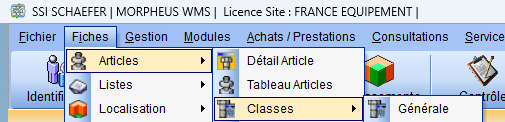
\includegraphics[width=0.7\linewidth]{images/mph_menu.png}
					\end{center}
					\caption{Partie du menu de l'application existante Morpheus}
					\label{fig:mph_menu}
				\end{figure}

				\begin{figure}[h!]
					\begin{center}
						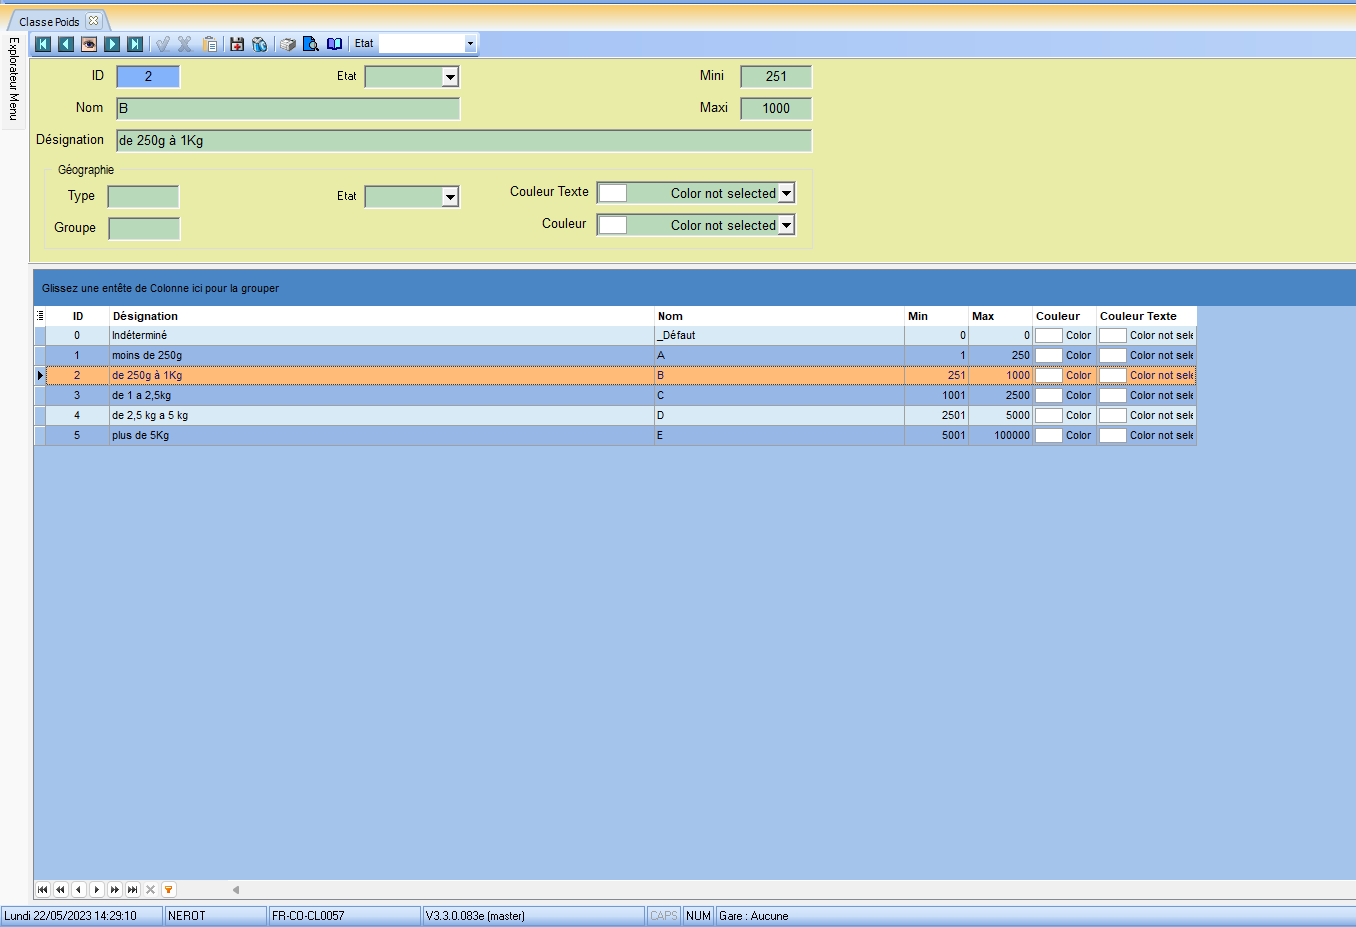
\includegraphics[width=0.7\linewidth]{images/mph_window.png}
					\end{center}
					\caption{Exemple d'une fenêtre de l'application existante Morpheus}
					\label{fig:mph_window}
				\end{figure}
		
		\newpage
		
		\section{Enjeux et importances}
			Au cours de mon stage au sein de SSI SCHÄFER, j'ai eu l'opportunité de travailler sur un projet d'une importance stratégique considérable. Ce projet n'était pas simplement une tâche parmi d'autres, mais il incarnait un défi clé que l'entreprise cherchait à relever pour atteindre ses objectifs à long terme. Dans cette section, je vais mettre en lumière les enjeux majeurs auxquels ce projet répondait et expliquer pourquoi sa réalisation revêtait une signification cruciale pour SSI SCHÄFER.\\

			Au-delà des aspects techniques, ce projet avait un impact direct sur la capacité de l'entreprise à prospérer dans un environnement concurrentiel en constante évolution. Il s'agissait d'une opportunité de consolider notre position sur le marché et de répondre aux attentes changeantes de nos clients. Tout au long de cette section, je vais détailler les aspects stratégiques et opérationnels qui ont rendu ce projet essentiel, ainsi que les résultats tangibles que nous avons pu obtenir grâce à notre travail acharné.\\

			En comprenant les enjeux et l'importance de ce projet, vous pourrez mieux apprécier la contribution significative que j'ai apportée à l'entreprise pendant mon stage, ainsi que la manière dont mes actions ont eu un impact direct sur ses objectifs globaux.
				
			\subsection{Enjeux du projet global}
				Chaque projet, qu'il soit grand ou petit, naît d'une nécessité, d'un défi ou d'un besoin spécifique. Mon expérience de stage au sein de SSI SCHÄFER m'a permis de plonger au cœur d'un projet passionnant, dont la genèse repose sur des enjeux initiaux essentiels. Cette section est dédiée à l'exploration de ces enjeux, qui ont été le point de départ de notre aventure collective.\\

				Lorsque nous envisageons un projet, il est essentiel de comprendre les raisons qui l'ont déclenché. Les enjeux initiaux sont les moteurs qui poussent une entreprise à investir des ressources, du temps et de l'énergie dans la réalisation d'un projet. Au travers de cette présentation, je vais vous plonger dans le contexte qui a entouré le lancement de ce projet, en expliquant les défis spécifiques, les besoins urgents et les opportunités à saisir.\\

				Au cours des prochaines sections, je vais détailler ces enjeux initiaux, identifier les problèmes qui se posaient, et montrer pourquoi il était impératif de mettre en place ce projet. Comprendre ces enjeux est la clé pour appréhender l'évolution du projet, les décisions prises en cours de route et les résultats obtenus. En saisissant les défis initiaux, vous serez en mesure de mesurer l'impact positif de notre travail dans la résolution de ces enjeux, et comment cela a contribué à l'entreprise ou à l'organisation.\\

					\subsubsection{Enjeux financiers}
						Le développement d'une application web Morpheus n'a pas pour premier enjeu un enjeu financier. En effet le projet a pour but de mener à une nouvelle communication sur le logiciel et offrir aux clients de nouvelles fonctionnalités.

						%\subsubsection{Coûts}
						%\subsubsection{Apports}
	
					\subsubsection{Enjeux stratégiques}
						Le projet a pour enjeux stratégiques de permettre à l'entreprise de communiquer sur la suite de logiciels morpheus et promouvoir de nouvelles fonctionnalités et un accès facilité à morpheus auprès des clients.

					\subsubsection{Enjeux humains}
						Le projet a pour enjeux humains de permettre aux clients d'accèder à Morpheus pour faire des opérations de gestion, directement depuis les bureaux, sans avoir à être en entrepôt et ce sans avoir à installer de client lourd mais seulement avoir besoin d'un navigateur web.

				%dans le cas de morpheus le passage à un client web n'a pas un objectif financier néanmoins on peut supposer que dans d'autres cas il y aurait une envie de faire plus de profits, revendre un logiciel, passer moins de temps à installer et configurer.. mais pour les clients..	
				
				\subsection{Objectifs globaux}
					Dans cette section, nous nous pencherons sur les objectifs globaux de notre projet, une étape fondamentale pour éclairer notre chemin vers la réalisation de nos aspirations. Ces objectifs constituent les piliers qui soutiendront notre initiative du début à la fin, et ils définissent la vision que nous cherchons à concrétiser. Nous parlerons ici des objectifs du projet global, nous reviendrons sur les objectifs du projet réalisé au cours du stage après dans le mémoire.\\

					Les objectifs globaux d'un projet vont bien au-delà de simples déclarations d'intention. Ils sont les fondations sur lesquelles repose chaque décision, chaque action et chaque ressource allouée. Ils servent de boussole, nous guidant à travers les complexités inhérentes à tout projet. Dans cette section, nous clarifierons ces objectifs, expliquerons leur pertinence et détaillerons leur rôle central dans la réussite globale de notre entreprise.
					
					Voici donc les objectifs globaux du projet :
					\begin{itemize}
						\bdot{Développer un client web morpheus (à partir du client lourd existant)}
						\bdot{Rendre morpheus plus accessible}
						\bdot{Créer un nouveau design ergonomique pour morpheus}
						\bdot{Faire une application web responsive accessible depuis n'importe quel terminal}%mettre définition terminal.. dans glossaire
					\end{itemize}

				%Présentez les objectifs clés du projet tels qu'ils ont été définis initialement. Quels étaient les résultats attendus ? Comment ces objectifs étaient-ils alignés sur la résolution des enjeux identifiés ?
				
				\subsection{Enjeux du projet de stage}
	%dire que les enjeux du projet de stage est d'établir un bon point de départ pour le projet global..
					%Le principal enjeu du projet de stage était de tester les différents possibilités de développement du projet ainsi que de poser des bases solides pour pouvoir le continuer sur la durée.

					Le principal enjeu du projet de stage consistait à explorer diverses possibilités de développement pour le projet et à établir des fondations solides en vue de sa poursuite à long terme.


				\subsection{Objectifs du projet de stage}
					%présenter sommairement et dire qu'on revient dessus plus en détail après..
					Voici une présentation sommaire des objectifs du projet de stage sur lesquels nous reviendrons par la suite.
					\begin{itemize}
						\bdot{Tester les outils de développement}
						\bdot{Créer une maquette}
						\bdot{Créer une première version de l'application web}
					\end{itemize}

				%\subsection{Parties prenantes et intervenants}
					%Indiquez les principales parties prenantes du projet, à la fois internes (collègues, départements) et externes (clients, partenaires). Identifiez les rôles des différentes personnes impliquées dans le projet.
					%\subsubsection{Monsieur Laurent GOURDON:Directeur général France}
					
					%\subsubsection{Monsieur Thierry NEROT:chef de projet;développeur du nouveau client lourd mopheus..}

					%\subsubsection{Collègues}

					%\subsubsection{Utilisateurs finaux de morpheus}
				
				\subsection{Contraintes et limitations du projet de stage}
					Tout projet, qu'il soit de petite ou de grande envergure, est confronté à des contraintes et à des limitations qui peuvent influencer sa planification, son exécution et ses résultats. Dans cette section, nous allons explorer les défis et les restrictions spécifiques auxquels nous avons dû faire face tout au long de notre projet.\\

					La reconnaissance et la gestion des contraintes et des limitations sont essentielles pour une gestion de projet efficace. Ces facteurs peuvent être de nature diverse, qu'il s'agisse de contraintes budgétaires, de délais serrés, de ressources limitées, de contraintes techniques, ou d'autres obstacles potentiels. Dans cette partie, nous allons détailler les contraintes et les limitations qui ont marqué notre projet et expliquer comment nous les avons abordées.\\

					Nous examinerons la manière dont ces contraintes ont influencé notre planification, nos décisions et nos actions, ainsi que les stratégies que nous avons déployées pour les surmonter. Nous mettrons également en évidence les leçons que nous avons tirées de ces contraintes en matière de gestion de projet.
					
					\subsubsection{Contraintes de délai}
						L'une des contraintes cruciales auxquelles nous avons été confrontés pendant ce stage était la durée limitée qui nous était accordée pour accomplir nos missions et atteindre les objectifs du projet. Le stage était fixé à une période de 27 semaines, ce qui représentait un défi en termes de planification et d'exécution.\\

						\paragraph{Durée fixe du stage\\}
							Conformément aux exigences de l'établissement d'enseignement et de l'entreprise d'accueil, le stage était prévu pour une durée fixe de 27 semaines. Cette contrainte temporelle était immuable et ne pouvait pas être prolongée.

						\paragraph{Complexité du projet\\}
							Le projet sur lequel nous avons travaillé était d'une certaine complexité, avec des objectifs ambitieux à atteindre. Cette complexité a rendu la gestion du temps d'autant plus cruciale.

						\paragraph{Apprentissage et conception initiale\\}
							Une période initiale était nécessaire pour nous familiariser avec l'entreprise, ses processus, et les spécificités du projet. Cela signifiait que nous disposions en réalité de moins de temps pour la phase active de développement.

						\paragraph{Solutions\\}
						\noindent
							Face à cette contrainte de durée, nous avons adopté une approche stratégique pour maximiser notre efficacité :

							\subparagraph{Planification avancée\\}
								Dès le début du stage, nous avons élaboré un plan détaillé, en identifiant les tâches essentielles à accomplir et en les répartissant sur la période disponible.

							\subparagraph{Priorisation des tâches\\}
								Nous avons établi des priorités claires en fonction des objectifs du projet et de leur importance stratégique, afin de nous concentrer sur les éléments les plus critiques en premier.\\

				Malgré la contrainte de durée du stage, nous avons réussi à atteindre nos objectifs en nous concentrant sur l'efficacité, la planification minutieuse et la gestion rigoureuse du temps. Cette expérience nous a permis d'acquérir des compétences précieuses en gestion du temps et en prise de décision stratégique.

					\subsubsection{Limitations en ressources humaines}
						%Présentez les limitations liées aux ressources humaines, telles que des équipes réduites, des compétences spécifiques manquantes, ou des membres d'équipe surchargés.
						Une des principales limitations auxquelles nous avons été confrontés tout au long de ce stage était liée aux ressources humaines. L'équipe de développeurs est composé uniquement de cinq personnes.
						
						\paragraph{Effectif limité\\}
							
						
						\paragraph{Surcharge de travail\\}
							Nous pouvons ici indiquer que l'équipe de développeurs est composé seulement de cinq personnes qui ont toutes déjà un emploi du temps chargé et que même si elles étaient là pour m'épauler globalement j'ai travaillé tout seul sur le projet. Donner exemple Thierry qui n'avait pas le temps de faire l'api..
						
						\paragraph{Solutions\\}
											

					\subsubsection{Conclusion}
							Au cours de ce projet, nous avons été confrontés à un ensemble varié de contraintes et de limitations, chacune apportant son propre défi. Cependant, au lieu de voir ces contraintes comme des obstacles insurmontables, nous les avons abordées comme des opportunités d'apprentissage et de croissance.\\

							La gestion des contraintes, des délais serrés, des ressources humaines limitées, et d'autres défis nous a permis de développer des compétences essentielles en gestion de projet, en résolution de problèmes, et en collaboration. Ces expériences nous ont montré que, même lorsque les ressources sont limitées, une planification minutieuse, une communication efficace, et une approche stratégique peuvent conduire à des résultats réussis.\\

							En fin de compte, la gestion des contraintes et des limitations a été une expérience formatrice qui a renforcé notre compréhension de la réalisation de projets dans des conditions du monde réel. Nous sommes fiers des résultats que nous avons obtenus malgré ces défis, et nous sommes convaincus que ces compétences acquises nous seront bénéfiques dans nos futures entreprises professionnelles.

			\subsection{Synthèse des enjeux et de l'importance}
				%Terminez cette section en faisant une synthèse des enjeux majeurs et de l'importance globale du projet pour l'entreprise. Récapitulez brièvement pourquoi ce projet était essentiel.

		\newpage

		\section{Méthodologie et outils}
			La réussite d'un projet repose souvent sur une méthodologie solide et l'utilisation adéquate d'outils appropriés. Au cours de mon stage au sein de SSI SCHÄFER, j'ai eu l'opportunité de travailler sur un projet stimulant qui nécessitait une approche réfléchie et une utilisation judicieuse des ressources technologiques. Dans cette section, je vais vous présenter la méthodologie que nous avons adoptée pour mener à bien ce projet ainsi que les outils technologiques qui ont été essentiels à sa réalisation.\\

			La méthodologie que nous avons choisie pour aborder ce projet a joué un rôle déterminant dans notre capacité à atteindre nos objectifs de manière efficace et efficiente. De plus, les outils que nous avons sélectionnés ont facilité la gestion, la collaboration et la mise en œuvre de ce projet complexe. En comprenant la méthodologie et les outils que nous avons utilisés, vous aurez une vision plus précise de la manière dont nous avons planifié et exécuté ce projet avec succès.\\

			Au fil de cette section, je vais détailler notre approche méthodologique, expliquer comment nous avons choisi les outils technologiques appropriés et démontrer comment cette combinaison a contribué à la réalisation de ce projet d'envergure.

			\subsection{Méthodologie adoptée}
				%Dans cette sous-partie, détaillez la méthodologie spécifique que vous avez adoptée pour aborder le projet. Expliquez pourquoi cette méthodologie a été choisie et comment elle était adaptée aux besoins du projet.
				La réalisation de tout projet réussi repose sur une méthodologie solide et des approches bien définies. Dans cette section, nous allons plonger dans les détails de la méthodologie que nous avons adoptée pour concevoir, développer et mettre en œuvre notre projet.\\

				La méthodologie est un cadre structuré qui guide chaque étape du processus, de la planification à la livraison du produit final. Elle permet d'assurer la cohérence, la qualité et la maîtrise tout au long du parcours.\\

				Dans cette partie, nous allons présenter la méthodologie spécifique que nous avons choisie, expliquer pourquoi elle était adaptée à notre projet, et détailler comment elle a influencé notre planification, notre conception, notre développement, notre mise en œuvre, et nos tests.\\

				Nous examinerons également les avantages de l'utilisation de cette méthodologie, les défis auxquels nous avons été confrontés, et les leçons que nous avons tirées de cette expérience en matière de gestion de projet.\\

				La méthodologie adoptée a été un élément clé de notre succès, en nous aidant à maintenir la structure, la cohérence et la qualité tout au long du processus. Cette section jettera les bases pour la suite de la présentation, où nous explorerons les résultats obtenus grâce à l'application de cette méthodologie.\\
				
				\subsubsection{Choix de la méthodologie:méthode en V}

				\subsubsection{Étapes de la méthodologie}
			
			
			\subsection{Planification et gestion de projet}
				%diagramme de gantt.. Expliquez comment le projet a été planifié et géré du début à la fin. Cela peut inclure des informations sur la définition des objectifs, la planification des étapes, la gestion des ressources, la budgétisation, et la gestion des risques.
				Au cœur de tout projet réussi réside une planification minutieuse et une gestion efficace. Dans cette section, nous allons plonger dans les détails de la manière dont notre projet a été structuré, planifié et géré pour atteindre ses objectifs.\\

				La planification et la gestion de projet sont des éléments cruciaux qui guident chaque étape de notre travail. Elles nous permettent d'établir des fondations solides, de définir des priorités, de gérer les ressources et de maintenir le cap tout au long du parcours. Dans cette partie, nous allons explorer les principes et les pratiques que nous avons mis en place pour assurer le succès de notre projet.\\

				Nous allons détailler la phase de planification, expliquer comment nous avons élaboré notre plan de projet, identifié les étapes clés et les jalons, et défini les ressources nécessaires. Nous aborderons également la gestion quotidienne du projet, y compris la manière dont nous avons suivi les progrès, résolu les problèmes et pris des décisions pour maintenir le projet sur la bonne voie.\\

				Chaque aspect de la planification et de la gestion de projet a contribué à notre capacité à atteindre nos objectifs, à respecter les délais et à maintenir la qualité de notre travail. En comprenant ces processus, vous aurez une vue d'ensemble claire de la façon dont notre projet a été dirigé du début à la fin.\\

				\subsubsection{Planification}
					Phases initiales du projet :
					\begin{itemize}
						\bdot{Installation et configuration des outils}
						\bdot{Expérimentation des outils}
						\bdot{Rédaction détaillée des besoins}
						\bdot{Développement du nouveau client html5}
						\bdot{Test et recettage du nouveau client}
						\bdot{Livraison}
					\end{itemize}

				\subsubsection{Diagramme de GANTT}

				\subsubsection{Budgétisation}
					Le budget du projet est composé des éléments suivants :
					\begin{itemize}
						\bdot{Investissement des outils tms software : 1800€}
						\bdot{25 semaines * 5 jours * 750€ : budget temps passé au développement}
						\bdot{7 semaines * 1 jour * 950€ : budget temps passé au management}
					\end{itemize}
			
			\subsection{Outils de gestion de projets}
				%Présentez les outils de gestion de projet que vous avez utilisés pour suivre et organiser les activités du projet. Cela peut inclure des logiciels de gestion de tâches, des diagrammes de Gantt, des	 tableaux de bord, etc.

				La gestion de projet moderne repose sur l'utilisation d'outils et de technologies qui facilitent la planification, le suivi et l'exécution des tâches. Dans cette section, nous allons explorer les outils de gestion de projet que nous avons utilisés pour optimiser notre efficacité et notre productivité tout au long de notre mission.\\

				Dans cette partie, nous allons présenter les outils que nous avons choisis et expliquer pourquoi ils étaient adaptés à nos besoins spécifiques. Nous allons décrire comment ces outils ont été intégrés dans notre processus de gestion de projet, comment ils ont facilité la collaboration entre les membres de l'équipe, et comment ils ont contribué à maintenir le projet sur la bonne voie.

				\subsubsection{Définitions}
				\subsubsection{Diagrammes de GANTT}
				\subsubsection{Confluence:outil de gestion de la documentation}
				
			\subsection{Collaboration et communication}
				La réussite d'un projet ne repose pas seulement sur la qualité de la planification et de l'exécution, mais également sur la manière dont les membres de l'équipe collaborent et communiquent. Dans cette section, nous allons explorer comment la collaboration efficace et la communication transparente ont été des piliers de notre réussite tout au long de ce projet.\\

				Dans cette partie, nous allons détailler les méthodes, les outils et les pratiques que nous avons utilisés pour favoriser la collaboration au sein de l'équipe et avec nos partenaires. Nous examinerons également comment la communication a été structurée pour assurer la circulation fluide de l'information.

				\subsubsection{Teams:outil de messagerie instantanée}%https://fr.wikipedia.org/wiki/Microsoft_Teams
					Microsoft Teams est une plateforme de collaboration et de communication professionnelle développée par Microsoft. Elle permet aux équipes de travail de collaborer en temps réel, que ce soit au sein d'une même entreprise ou entre différentes organisations. Microsoft Teams offre une gamme de fonctionnalités, notamment la messagerie instantanée, la vidéoconférence, le partage de fichiers, la gestion de tâches, l'intégration d'applications tierces, et bien plus encore.
					
					%Teams est vraiment très utile pour communiquer rapidement avec les collègues, surtout quand ils sont en télétravail. Cela est aussi très pratique pour faire des réunions en ligne. Au cours de mon stage j'ai principalement utilisé Teams pour ces deux fonctionnalités.
					Teams s'avère extrêmement pratique pour faciliter la communication avec les collègues, particulièrement lorsqu'ils travaillent à distance. De plus, il sert de manière très commode pour la tenue de réunions en ligne. Pendant mon stage, j'ai principalement eu recours à Teams pour exploiter ces deux fonctionnalités.

				\subsubsection{Outlook:outil de messagerie}%https://fr.wikipedia.org/wiki/Microsoft_Outlook
					Outlook est un client de messagerie électronique qui permet aux utilisateurs de gérer leurs e-mails, leurs calendriers, leurs tâches, leurs contacts et leurs notes en un seul endroit. Il offre un ensemble de fonctionnalités qui facilitent la communication, la planification et l'organisation de tâches professionnelles et personnelles. Les principales caractéristiques d'Outlook comprennent la réception et l'envoi d'e-mails, la gestion des calendriers pour planifier des rendez-vous et des réunions, la création de tâches pour suivre les activités à accomplir, la gestion des contacts pour organiser les informations de contact, et la possibilité de prendre des notes.

					%Durant mon stage, Outlook m'a principalement servi à envoyer des mails à mes collègues ainsi que Monsieur Hamrioui. Il m'a aussi permis de planifier certaines tâches, rendez-vous et réunions sur le calendrier inclus à l'application.
					Pendant mon stage, j'ai principalement utilisé Outlook pour l'envoi de courriels à mes collègues et à Monsieur Hamrioui. De plus, j'ai profité de ses fonctionnalités pour planifier diverses tâches, rendez-vous et réunions grâce au calendrier intégré dans l'application.

				\subsubsection{"Point dev":réunion hebdomadaire}
					Toutes les semaines, vendredi à 14, nous effectuions une réunion, appelée "Point dev", qui réunissait tous les développeurs de l'entreprise. Durant cette réunion, chachun indiquait ce qu'il avait fait pendant la semaine écoulée et pouvait parler des problèmes rencontrés. Cela permettait aussi de trouver des solutions aux problèmes évoqués.

				\subsubsection{Réunions ponctuelles}
					Parfois nous faisions des réunions avec Monsieur GOURDON et Monsieur NEROT afin de parler de l'avancement du projet et vérifier qu'il avancait toujours dans la bonne direction.

				\subsubsection{Communication avec les collègues}
					Bien que j'étais principalement seul à travailler sur le projet, je pouvais, si besoin, discuter avec mes collègues des problèmes rencontrés et chercher ensemble une solution. La communication avec eux a toujours été facile et fluide et partcipait à la bonne réussite du projet.
			
			%\subsection{Méthodes de développement}
				%Si votre projet impliquait du développement logiciel ou une création de produit, expliquez les méthodes spécifiques que vous avez utilisées. Par exemple, Agile, Scrum, Waterfall, ou d'autres approches adaptées à votre contexte.

				%La réalisation d'un projet réussi exige une approche méthodique et réfléchie pour la conception, le développement et l'implémentation. Dans cette section, nous allons plonger dans les méthodes de développement que nous avons utilisées pour donner vie à notre projet.\\

				%Dans cette partie, nous allons présenter les méthodes que nous avons choisies et expliquer pourquoi elles étaient adaptées à notre projet spécifique. Nous allons détailler comment ces méthodes ont influencé la planification, la conception, la mise en œuvre et les tests de notre projet.
			
			\subsection{Outils technologiques}				
				Les avancées technologiques ont transformé la manière dont nous concevons, développons et mettons en œuvre des projets. Dans cette section, nous allons explorer les outils technologiques que nous avons exploités pour donner vie à notre projet et atteindre nos objectifs.\\

				Dans cette partie, nous allons présenter les outils technologiques spécifiques que nous avons utilisés, en expliquant pourquoi nous les avons choisis et comment ils se sont intégrés dans notre démarche globale. Nous allons détailler comment ces outils ont contribué à la réalisation de nos objectifs et comment ils ont amélioré notre efficacité tout au long du projet.

				\subsubsection{Delphi}%https://fr.wikipedia.org/wiki/Delphi_(langage)
					Delphi est à la fois un langage de programmation orienté objet et un environnement de développement intégré (EDI) pour ce langage. Delphi est un EDI propriétaire fonctionnant sous Windows créé en 1995 par Borland. Delphi embarque une version orientée objet du langage Pascal : le Pascal Objet, renommé Langage de programmation Delphi au fil des modifications apportées par Borland.

					Dans le cadre de notre projet, Delphi a été le premier langage de programmation envisagé pour réaliser l'application web Morpheus. Avec l'utilisation du framework TMS Web de TMS Software, nous avons pu créer la première version de l'application web

					\paragraph{TMS Software et TMS Web\\}
						%https://www.tmssoftware.com/site/default.asp
						%https://www.tmssoftware.com/site/tmswebcoreintro.asp
						
		
					D'abord envisagé parce que déjà utilisé par l'entreprise, cet outil technologique nous a permis de nous rendre compte qu'il n'était pas le plus adapté pour le projet et a participé au choix d'une technologie plus adapté.

				\subsubsection{HTML}%https://fr.wikipedia.org/wiki/Hypertext_Markup_Language
					Le HyperText Markup Language, couramment abrégé en HTML, représente le langage de balisage conçu pour la création de pages web.\\

					%en annexe ou glossaire définition hypertexte..
					Ce langage permet la rédaction d'hypertexte, la structuration sémantique des pages web, la mise en forme de contenu, la création de formulaires interactifs et l'intégration de ressources multimédias telles que des images, des vidéos et des scripts informatiques. L'HTML offre également la possibilité de créer des documents compatibles avec une grande variété de dispositifs, en respectant les normes d'accessibilité du web.				
				
				\subsubsection{CSS}%https://fr.wikipedia.org/wiki/Feuilles_de_style_en_cascade
					Les feuilles de style en cascade, souvent abrégées en CSS à partir de l'anglais Cascading Style Sheets, représentent un langage informatique utilisé pour définir la mise en forme des documents HTML et XML.
					
				\subsubsection{Javascript}%https://fr.wikipedia.org/wiki/JavaScript
					JavaScript est un langage de programmation de scripts principalement employé dans les pages web interactives et à ce titre est une partie essentielle des applications web. Avec les langages HTML et CSS, JavaScript est au cœur des langages utilisés par les développeurs web. Une grande majorité des sites web l'utilisent, et la majorité des navigateurs web disposent d'un moteur JavaScript pour l'interpréter.

					\paragraph{ReactJS}
						%https://fr.wikipedia.org/wiki/React
						%https://react.dev/
	
						%glossaire pour des mots comme DOM.. plus mettre plus d'infos en annexe.. nodejs...

						React (également connu sous le nom de React.js ou ReactJS) est une bibliothèque JavaScript open source développée par Facebook (aujourd'hui Meta) à partir de 2013. L'objectif principal de cette bibliothèque est de simplifier la création d'applications web monopages en permettant la création de composants dépendants de l'état, qui génèrent une page (ou une portion de page) HTML à chaque modification de cet état.\\

						React se concentre exclusivement sur la gestion de l'interface utilisateur de l'application, considérée comme la vue dans le modèle MVC (Modèle-Vue-Contrôleur). Par conséquent, elle peut être utilisée en combinaison avec d'autres bibliothèques ou frameworks MVC tels qu'AngularJS. Ce qui distingue cette bibliothèque de ses concurrentes, c'est sa flexibilité et ses performances. Elle travaille avec un DOM virtuel et met à jour le rendu dans le navigateur uniquement lorsque cela est nécessaire, ce qui contribue à améliorer les performances de l'application.

					\paragraph{DevExtreme par DevExpress\\}
					
					%https://js.devexpress.com/

				\subsubsection{Git}%https://fr.wikipedia.org/wiki/Git
					Git est un logiciel de gestion de versions décentralisé. Dans le projet, il nous a principalement servi a faire une sauvegarde régulière du code produit.%en annexe expliquer logiciel de gestion de versions décentralisé..

				\subsubsection{Insomnia}%https://insomnia.rest/
					Insomnia, est une plateforme open-source de Kong Inc. (en) pour tester des API. Cet outil nous a permis de tester des requêtes sur l'API que nous avons créé sans avoir besoin de développer quoi que ce soit.

				\subsubsection{Microsoft SQL Server \& Microsoft SQL Server Management Studio}%https://fr.wikipedia.org/wiki/Microsoft_SQL_Server
				%https://en.wikipedia.org/wiki/SQL_Server_Management_Studio

					\paragraph{Microsoft SQL Server\\}
						Microsoft SQL Server est un système de gestion de base de données (SGBD) en langage SQL incorporant entre autres un SGBDR (SGBD relationnel »).

					\paragraph{Microsoft SQL Server Management Studio\\}
						Microsoft SQL Server Management Studio (SSMS) est une application logicielle développée par Microsoft qui est utilisée pour configurer, gérer et administrer tous les composants au sein de Microsoft SQL Server.

					Ces outils technologiques sont donc la base pour nous de notre base de données.

				\subsubsection{Visual Studio Code}%https://fr.wikipedia.org/wiki/Visual_Studio_Code
					Visual Studio Code est un éditeur de code extensible développé par Microsoft pour Windows, Linux et macOS. Les fonctionnalités incluent la prise en charge du débogage, la mise en évidence de la syntaxe, la complétion intelligente du code (IntelliSense.), les snippets, la refactorisation du code et Git intégré. Les utilisateurs peuvent modifier le thème, les raccourcis clavier, les préférences et installer des extensions qui ajoutent des fonctionnalités supplémentaires.\\

					Visual Studio Code est l'éditeur de code que j'utilise de nombreuses années, je sais donc assez bien comment l'utiliser. Il a donc été évident pour moi de l'utiliser dans ce projet afin d'être le plus productif possible et de ne pas perdre de temps à prendre en main un nouvel éditeur de code.
					
				\subsubsection{Modelio}%https://en.wikipedia.org/wiki/Modelio
					Modelio est un outil de modélisation UML. Il m'a notamment servi à créer le diagramme de classe des nouvelles tables de la base de données.

				\subsubsection{Latex}%https://fr.wikipedia.org/wiki/LaTeX
					LaTeX (dont le logo est LATEX) est un langage et un système de composition de documents. Il s'agit d'une collection de macrocommandes destinées à faciliter l'utilisation du « processeur de texte » TeX de Donald Knuth. J'ai notamment utilisé Latex pour la rédaction de ce mémoire ainsi que des rapports d'avancements durant tout le stage.			

			%\subsection{Évaluation de l'efficacité}%Terminez en expliquant comment l'utilisation de la méthodologie et des outils a contribué à l'efficacité du projet. Vous pouvez mentionner des exemples de résultats positifs ou d'améliorations dans la gestion et la réalisation du projet.
		
		\newpage

		\section{Déroulement du projet}
			Le succès d'un projet repose non seulement sur son objectif et ses outils, mais également sur la manière dont il est planifié, exécuté et géré tout au long de son cycle de vie. Au cours de mon stage au sein de SSI SCHÄFER, j'ai eu l'opportunité de participer à un projet d'envergure qui a nécessité une planification minutieuse et une exécution rigoureuse. Dans cette section, je vais vous plonger dans le déroulement complet de ce projet, en décrivant les différentes étapes, les jalons importants, et la manière dont nous avons géré les défis et les opportunités tout au long de ce parcours.\\

			Le projet que j'ai eu l'honneur de contribuer avait un impact significatif sur l'entreprise, et sa réalisation nécessitait une coordination efficace, une communication transparente et une gestion attentive des ressources. En comprenant les étapes par lesquelles nous sommes passés, vous pourrez mieux apprécier la complexité de ce projet, ainsi que la manière dont nous avons surmonté les obstacles pour atteindre nos objectifs.\\

			Au fil de cette section, je vais détailler comment le projet a été organisé, comment nous avons géré les ressources, les délais et les risques, ainsi que les leçons que nous avons tirées de cette expérience. En explorant le déroulement complet de ce projet, vous aurez une vue d'ensemble complète de notre démarche pour atteindre le succès.


			\subsection{Objectifs et planification initiale}
				%Dans cette sous-partie, détaillez les objectifs du projet tels qu'ils ont été initialement définis. Expliquez comment le projet a été planifié en termes de ressources, de délais et d'étapes préliminaires. Présentez le contexte initial.

				La clarté des objectifs et la planification méthodique sont les fondements de tout projet réussi. Dans cette section, nous allons explorer les objectifs que nous nous sommes fixés au début de notre projet et la planification initiale qui a guidé nos actions.\\

				Le processus de définition des objectifs est une étape fondamentale dans la réalisation de tout projet. Ces objectifs servent de boussole, nous orientant vers nos buts et nous aidant à mesurer notre succès tout au long du parcours. Dans cette partie, nous allons détailler ces objectifs, expliquer pourquoi ils ont été choisis, et comment ils étaient alignés sur les enjeux et les besoins que nous avons identifiés précédemment.\\

				La planification initiale est tout aussi essentielle. Elle nous permet de définir la trajectoire du projet, d'identifier les étapes clés, les ressources nécessaires, et de fixer des échéances réalistes. Dans cette section, nous allons décrire comment nous avons élaboré notre plan initial, en mettant en lumière les décisions clés prises pour assurer le succès du projet.\\

				En comprenant ces éléments, vous aurez une vue d'ensemble claire de la manière dont notre projet a été conçu et structuré pour atteindre des objectifs spécifiques, tout en tenant compte des contraintes et des réalités du terrain. Cette partie jettera les bases pour la suite du mémoire, où nous détaillerons notre mise en œuvre et nos résultats par rapport à ces objectifs initiaux.

				\subsubsection{Objectifs}
					Les objectifs initiaux du projet étaient les suivants :
	
					\begin{itemize}
						\bdot{Develop a morpheus client in full HTML 5 and responsive for some windows of the existing Mopheus client}
						\bdot{Experiment the development tools of TMS Web}
						\bdot{Make a UI mockup}
							\begin{itemize}
								\bdotoutlined{Main window}
									\begin{itemize}
										\bsquare{Menu}
											\begin{itemize}
												\bsquareoutlined{Icons}
												\bsquareoutlined{Style (as windows' style : colors)}
												\bsquareoutlined{X configurable levels and sub levels}
													\begin{itemize}
														\bdiamond{From a database : display or not some menu entries}
													\end{itemize}
											\end{itemize}
										\bsquare{Function buttons}
											\begin{itemize}
												\bsquareoutlined{Style}
												\bsquareoutlined{Icons}
												\bsquareoutlined{Size of buttons (16, 32 or 48)}
												\bsquareoutlined{Make buttons visible or not}
												\bsquareoutlined{Buttons layout depending of the number : alignements..}
											\end{itemize}
										\bsquare{Treeview}
											\begin{itemize}
												\bsquareoutlined{Style}
												\bsquareoutlined{Icons (in front of the label with touching triangle)}
												\bsquareoutlined{Display a list over a level following a request}
												\bsquareoutlined{Dynamically load of trees}
													\begin{itemize}
														\bdiamond{Configuration to make the trees visible or not}
													\end{itemize}
											\end{itemize}
									\end{itemize}
								\bdotoutlined{Style management}
								\bdotoutlined{MDI multi-window management (tabs)}
									\begin{itemize}
										\bsquare{Icons}
										\bsquare{Can be closed or not with a cross}
									\end{itemize}
								\bdotoutlined{Modal window management}
									\begin{itemize}
										\bsquare{Cross to close the window visible or not}
										\bsquare{Position memory}
									\end{itemize}
								\bdotoutlined{Login}
								\bdotoutlined{Database connection}
							\end{itemize}
						\bdot{Write a description of the client's operating mode at the ergonomic level}
						\bdot{Develop a first version with basic windows}
							\begin{itemize}
								\bdotoutlined{Main window}
									\begin{itemize}
										\bsquare{Menu}
											\begin{itemize}
												\bsquareoutlined{Icons}
												\bsquareoutlined{Style (as windows' style : colors)}
												\bsquareoutlined{X configurable levels and sub levels}
													\begin{itemize}
														\bdiamond{From a database : display or not some menu entries}
													\end{itemize}
											\end{itemize}
										\bsquare{Function buttons}
											\begin{itemize}
												\bsquareoutlined{Style}
												\bsquareoutlined{Icons}
												\bsquareoutlined{Size of buttons (16, 32 or 48)}
												\bsquareoutlined{Make buttons visible or not}
												\bsquareoutlined{Buttons layout depending of the number : alignements..}
											\end{itemize}
										\bsquare{Treeview}
											\begin{itemize}
												\bsquareoutlined{Style}
												\bsquareoutlined{Icons (in front of the label with touching triangle)}
												\bsquareoutlined{Display a list over a level following a request}
												\bsquareoutlined{Dynamically load of trees}
													\begin{itemize}
														\bdiamond{Configuration to make the trees visible or not}
													\end{itemize}
											\end{itemize}
									\end{itemize}
								\bdotoutlined{Style management}
								\bdotoutlined{MDI multi-window management (tabs)}
									\begin{itemize}
										\bsquare{Icons}
										\bsquare{Can be closed or not with a cross}
									\end{itemize}
								\bdotoutlined{Modal window management}
									\begin{itemize}
										\bsquare{Cross to close the window visible or not}
										\bsquare{Position memory}
									\end{itemize}
								\bdotoutlined{Login}
								\bdotoutlined{Database connection}
								\bdotoutlined{Access rights management}
								\bdotoutlined{Windows configuration management in xml}
									\begin{itemize}
										\bsquare{Window type}
										\bsquare{Associated grid}
										\bsquare{SQL query}
									\end{itemize}
							\end{itemize}
					\end{itemize}

				\subsubsection{Planification initiale}
					%gantt..
						
			\subsection{Étapes du projet}
				La réalisation d'un projet réussi nécessite un plan solide et une exécution méthodique. Dans cette section, nous allons explorer les étapes clés qui ont jalonné notre parcours, du début à la fin du projet. Cette chronologie nous permettra de comprendre la séquence logique de notre travail et les accomplissements qui ont marqué chaque phase.\\

				La gestion des étapes d'un projet est essentielle pour assurer la cohérence, l'efficacité et la maîtrise des délais. Chaque étape représente un ensemble spécifique de tâches, d'objectifs et de livrables qui nous rapprochent de la réalisation de notre mission globale. Au cours de cette section, nous allons détailler ces étapes et expliquer comment elles étaient alignées sur nos objectifs initiaux.

		%\subsection{Architecture de l'application}
			%schéma de l'architecture de l'application

		%\subsection{Système de gestion de bases de données (SGBD)}
			%Le système de gestion de bases de données utilisé par Morpheus est MSSqlServer développé par Microsoft. On peut notamment accéder aux bases de données via l'outil Microsoft SQL Server Management Studio.
			%Actuellement beaucoup d'informations utiles à Morpheus sont stockés dans une base de données, et pas seulement les données affichées aux utilisateurs mais aussi de nombreux paramètres de gestion des interfaces graphiques. Il existe aussi de nombreuses procédures stockées permettant d'effectuer certaines actions. À l'heure actuelle, nous ne souhaitons pas changer ce système, c'est ainsi qu'afin de pouvoir accéder aux informations contenues dans la base de données, nous avons décidé de mettre en place une API REST servant de solution back-end à l'application web. Néanmoins si nous nous rendons compte que l'adaptation ou la création de nouvelles tables permettent l'amélioration de l'application web, nous ferons les ajustements nécessaires.

				\subsubsection{Étape n°1 : Choix du langage de progammation pour le frontend}
					L'application front-end de l'application web Morpheus est sans doute la plus importante du projet. En effet, elle représente la partie interface graphique et sera donc celle avec laquelle l'utilisateur va interagir. Il parait donc logique que la première étape du projet soit de choisir le langage de programmation le plus adapté pour développer cette application.
	
					\paragraph{Solutions possibles\\}
						Trois principales solutions ont été envisagées pour convenir aux objectifs de ce projet. Nous allons voir quelles sont ces solutions et pourquoi elles ont été envisagés.
						%à voir utiliser subparagraph..
						\subparagraph{Delphi et TMS Software\\}
							Delphi et TMS Software ont été la première solution envisagée dans ce projet. En effet le langage delphi étant déjà utilisé au sein de l'entreprise SSI Schäfer, il a été logique pour eux de me proposer de réaliser le projet en utilisant cet outil. Néanmoins, nous nous sommes très vite rendu compte que cela n'allait pas être l'outil le plus adapté pour notre projet d'application web.%en annexe brève présentation de delphi et tms software + lien vers site ...
					%déjà utilisé par l'entreprise..
					
						\subparagraph{Javascript\\}
							Javascript a été la deuxième option a laquelle j'ai pensé pour faire ce projet.%en annexe brève présentation de javascript
									%JS vanilla
						\subparagraph{ReactJS et devextreme\\}%en annexe brève présentation de reactjs et devextreme
									%React JS + devextreme..						

					\paragraph{Comparatif technique entre TMS Web et DevExtreme\\}
							Voici un comparatif technique entre les solutions TMS Web et DevExtreme dans le cadre du développement d'une application web :\\
							\begin{enumerate}
								\item Langage de programmation
									\begin{itemize}
										\bdot{TMS Web se base sur le Pascal Objet, un langage de programmation orienté objet. Il est particulièrement adapté aux développeurs familiers avec Delphi ou Free Pascal. L'utilisation de Pascal Objet dans TMS Web offre une courbe d'apprentissage plus facile pour les développeurs Delphi.}
										\bdot{DevExtreme se base sur JavaScript, un langage incontournable pour le développement web. Cela signifie que les développeurs travaillent directement avec JavaScript et peuvent choisir d'utiliser des frameworks supplémentaires tels qu'Angular, React ou Vue.js pour développer l'application.}
									\end{itemize}

								\item Composants et widgets
									\begin{itemize}
										\bdot{TMS Web propose des composants et des widgets basés sur les principes de la bibliothèque VCL (Visual Component Library) de Delphi. Cela permet de créer des interfaces riches avec des fonctionnalités avancées.}
										\bdot{DevExtreme offre une large gamme de widgets prêts à l'emploi, allant des tableaux de bord interactifs aux graphiques, aux grilles, aux calendriers, etc. Ces widgets sont optimisés pour les performances et l'expérience utilisateur.}
									\end{itemize}
	
								\item Intégration et compatibilité
									\begin{itemize}
										\bdot{TMS Web est étroitement intégré à l'environnement Delphi. Il est conçu pour être utilisé principalement avec Delphi, ce qui offre une expérience de développement cohérente pour les utilisateurs existants de Delphi. Cependant, cela peut limiter la portabilité vers d'autres plates-formes.}
										\bdot{DevExtreme est indépendant de la plate-forme et peut être utilisé avec différents environnements de développement tels que Visual Studio Code, Angular, React, etc. Cela permet une plus grande flexibilité en termes de choix de la technologie et de la plate-forme.}
									\end{itemize}

								\item Licence et coûts
									\begin{itemize}
										\bdot{Les coûts de TMS Web sont souvent associés aux licences Delphi de TMS Software. Les prix varient en fonction des modules nécessaires et des licences Delphi choisies.}
										\bdot{DevExtreme propose différentes options de licence, y compris une version gratuite pour une utilisation non commerciale. Pour une utilisation commerciale ou l'accès à des fonctionnalités avancées, une licence payante peut être nécessaire.}
									\end{itemize}

								\item Performance
									\begin{itemize}
										\bdot{Les applications TMS Web peuvent bénéficier des optimisations et des performances liées à Delphi. Cependant, étant donné qu'il s'appuie sur le Pascal Objet, il peut y avoir des limites en termes de performances JavaScript (le Pascal Object étant traduit en JavaScript) par rapport aux concurrents JavaScript natifs.}
										\bdot{DevExtreme est optimisé pour les performances JavaScript et offre une expérience utilisateur réactive et fluide, en particulier dans les applications web modernes.}
									\end{itemize}

								\item Documentation et communauté :
									\begin{itemize}
										\bdot{TMS Web dispose d'une documentation et d'une communauté pour soutenir les développeurs, bien que la communauté soit potentiellement plus restreinte que celle des grands frameworks JavaScript.}
										\bdot{DevExtreme bénéficie du soutien de DevExpress, une entreprise bien établie, et propose une documentation complète et une communauté de développeurs JavaScript active et étendue.}
									\end{itemize}
		
								\item Avis/ressenti personnel
									\begin{itemize}
										\bdot{}
										\bdot{}
									\end{itemize}
							\end{enumerate}

						%Le choix entre TMS Web et DevExtreme dépend de facteurs tels que la familiarité avec le langage de programmation, l'intégration avec les environnements de développement existants, les besoins spécifiques en matière de fonctionnalités et de performances, ainsi que les coûts associés. Les développeurs Delphi expérimentés peuvent trouver TMS Web plus intuitif, tandis que DevExtreme offre une flexibilité accrue pour les projets multiplateformes et une large gamme de widgets modernes.
		
%Les sources utilisées sont les sites de tmssoftware et de devexpress + voir developpez commentaire..
		
						\paragraph{Solution retenue}
							%ReactJS .. + pourquoi
							La solution que nous avons décidé de retenir est ReactJS, en effet cette technologie est celle qui correspond le mieux à ce que nous souhaitons faire dans le cadre de ce projet.

%dire que si on avait réfléchi plutôt au langage/framework le plus adapté on aurait pu économiser les coûts de licences de delphi 11 + tms software...
%+ mon côté ingénieur est ressorti en apportant le fait que le langage choisi de base n'était pas le plus adapté...
			
				\subsubsection{Étape n°2 : Développement de la première version du frontend}
					Après avoir choisi le langage de programmation avec lequel nous voulions travailler, j'ai commencé à développer la première version du frontend de l'application web.
					
					%expliquer dev + diagramme de classe..
					
				\subsubsection{Étape n°3 : Développement d'un backend pour intéragir avec la base de données}
					%dire que Thierry devait faire une api mais qu'il avait moins le temps
					%j'ai donc décidé de développer mon api et je voulais aussi voir ce qu'il était possible de faire en js + que ça serait bien d'utiliser la même technologie que front..
			
			\subsection{Suivi et contrôle}
				Le suivi et le contrôle sont les piliers qui assurent la cohérence, la qualité et la maîtrise d'un projet tout au long de son déroulement. Dans cette section, nous allons plonger dans les détails de la manière dont nous avons suivi et contrôlé notre projet pour nous assurer qu'il restait aligné sur nos objectifs et respectait les normes de qualité.\\

				Le suivi et le contrôle sont des éléments essentiels de la gestion de projet, car ils permettent de maintenir le cap, de résoudre les problèmes en temps réel, et de prendre des décisions éclairées pour assurer le succès du projet. Dans cette partie, nous allons détailler les méthodes, les outils et les pratiques que nous avons utilisés pour suivre la progression, évaluer les résultats et maintenir la qualité de notre travail.

				\subsubsection{Réunion hebdomadaire:"Point dev"}
					Nous en avons parlé plutôt dans la section methodologie (mettre ref section..), le point est une réunion hebdomadaire où chaque développeur parle de ce qu'il a fait pendant la semaine. C'était donc l'occasion pour moi de présenter mon travail, ce qui assurait le suivi du projet et permettait de contrôler que le projet allait toujours dans la bonne direction.
					
				\subsubsection{Réunions ponctuelles de suivi}
					En tant que directeur général France de SSI SCHÄFER, Monsieur GOURDON a un emploi du temps très chargé. Néanmoins cela lui tenait a coeur de suivre l'évolution du projet de développement de l'application web. C'est donc pour cela que nous faisions parfois des réunions ponctuelles, le plus souvent avec Monsieur NEROT, qui me permettait de lui présenter mon travail et lui permettait, si besoin, de me donner ses indications sur la marche à suivre pour continuer le projet sur la bonne voie.
			%\subsection{Modifications et ajustements}
				%Si des changements ont été apportés au projet en cours de route, expliquez comment ils ont été gérés et documentés. Présentez les raisons de ces modifications et leur impact sur le projet.

		\newpage

		\section{Défis et solutions}
			%Identifiez les défis auxquels vous avez été confronté pendant le stage, que ce soit au niveau technique, organisationnel ou humain. Ensuite, détaillez les solutions que vous avez proposées pour les surmonter. Cela montre votre capacité à résoudre des problèmes.
			Tout projet, quelle que soit sa nature, est accompagné de son lot de défis et d'obstacles. Ces défis sont autant d'opportunités d'apprentissage et de croissance, et ils témoignent de la complexité inhérente à la réalisation de projets significatifs. Au cours de mon stage au sein de SSI SCHÄFER, j'ai eu l'occasion de faire face à des défis variés et stimulants dans le cadre du projet que j'ai contribué à mener à bien.\\

			Dans cette section, je vais vous présenter les défis que nous avons rencontrés tout au long du projet, qu'ils soient d'ordre technique, organisationnel ou stratégique. Je vais également vous expliquer comment nous avons travaillé en équipe pour identifier, analyser et élaborer des solutions efficaces pour surmonter ces défis.\\

			Le but de cette section n'est pas seulement de mettre en lumière les obstacles auxquels nous avons été confrontés, mais surtout de démontrer notre capacité à réagir de manière proactive et créative pour les résoudre. Chaque défi a été une occasion d'appliquer nos compétences, de prendre des décisions éclairées et d'adapter notre approche pour atteindre nos objectifs malgré les obstacles. En comprenant les défis que nous avons relevés et les solutions que nous avons apportées, vous aurez un aperçu de notre agilité et de notre détermination à réussir dans un environnement professionnel en constante évolution.

			\subsection{Cyberattaque au sein de l'entreprise}			
				%rappeler que schaefer est international
				%subit une cyberattaque
				%pas trop impacté de mon côté : expliquer un peu
				%mais télétravail (à voir)
				%plus j'ai vu l'impact sur les colllègues
				%plus yutz qui sont venus..

			%\subsection{Identifications des défis}
				%Dans cette sous-partie, présentez les défis spécifiques auxquels vous avez été confronté tout au long du projet. Décrivez les problèmes ou les obstacles qui se sont présentés.

			%\subsection{Contexte des défis}
				%Expliquez le contexte dans lequel chaque défi est survenu. Quelles circonstances ou facteurs ont contribué à ces problèmes ? Précisez l'impact de ces défis sur le projet.
					
			%\subsection{Analyse des défis}
				%Détaillez l'analyse que vous avez réalisée pour comprendre pleinement chaque défi. Quelles étaient les causes sous-jacentes ? Quels étaient les risques potentiels associés à ces défis ?
					
			%\subsection{Priorisation des défis}
				%Discutez de la manière dont vous avez hiérarchisé les défis en fonction de leur gravité et de leur impact sur le projet. Quels étaient les défis les plus critiques à résoudre en premier ?
				
			%\subsection{Solutions proposées}
				%Présentez les solutions que vous avez proposées pour surmonter chaque défi. Expliquez comment vous avez développé des plans d'action pour résoudre ces problèmes.
				
			%\subsection{Mise en oeuvre des solutions}
				%Détaillez comment vous avez mis en œuvre les solutions que vous avez proposées. Qui était responsable de leur exécution ? Quels étaient les délais pour les résoudre ?
				
			%\subsection{Résultats et impact}
				%Expliquez les résultats obtenus grâce à la mise en œuvre de chaque solution. Quels changements ou améliorations avez-vous observés ? Comment ces solutions ont-elles contribué au succès global du projet ?
				
			%\subsection{Apprentissage et adaptations}
				%Partagez les enseignements que vous avez tirés de la résolution de ces défis. Comment ces expériences vous ont-elles aidé à vous améliorer en tant que professionnel ? Quels ajustements avez-vous effectués dans votre approche pour éviter de futurs problèmes similaires ?
				
			%\subsection{Conclusion des défis et solutions}
				%Terminez en faisant une synthèse des défis majeurs que vous avez rencontrés tout au long du projet et de la manière dont vous les avez résolus avec succès. Réfléchissez sur la façon dont ces défis ont contribué à votre développement professionnel.
			
	%Chacune de ces sous-parties contribue à fournir une vue d'ensemble complète des défis et des solutions rencontrés tout au long du projet, tout en mettant en évidence votre capacité à résoudre des problèmes de manière efficace. Veillez à maintenir une structure logique pour faciliter la compréhension de votre démarche.

		\newpage

		\section{Réalisations et résultats}
			%Mettez en avant les réalisations concrètes que vous avez obtenues grâce à votre contribution au projet. Cela peut inclure des fonctionnalités développées, des processus améliorés, des gains d'efficacité chiffrés, ou même des impacts positifs sur l'entreprise, tels que des économies de coûts ou une meilleure satisfaction des clients.
			Au cœur de tout projet se trouvent les réalisations et les résultats qui attestent du succès et de la valeur d'une initiative. Au cours de mon stage au sein de SSI SCHÄFER, j'ai eu l'opportunité de contribuer activement à un projet qui a généré des réalisations significatives et des résultats tangibles. Dans cette section, je vais vous dévoiler ces réalisations et résultats, qui illustrent l'impact concret de notre travail sur le projet.\\

			Chacune des actions entreprises au cours de ce projet visait à atteindre des objectifs spécifiques, et ces objectifs étaient étroitement liés à la réussite de l'entreprise. Au-delà des défis et des obstacles rencontrés en chemin, ces réalisations et résultats reflètent notre engagement envers la réussite et notre capacité à transformer des idées en actions concrètes.\\

			Au fil de cette section, je vais mettre en avant les réalisations clés qui ont émergé de notre travail acharné, les résultats obtenus grâce à nos efforts collectifs, et l'impact positif de ces réalisations sur l'entreprise ou l'organisation. Je vais également illustrer comment ces réalisations ont contribué à l'atteinte des objectifs du projet.\\

			En comprenant les réalisations et les résultats de ce projet, vous aurez une vue complète de la valeur ajoutée que j'ai apportée en tant que stagiaire, ainsi que de l'impact concret de notre collaboration sur les objectifs globaux de l'entreprise. Ces réalisations témoignent de notre engagement envers l'excellence et de notre contribution à la réussite de l'entreprise.

			\subsection{Objectifs atteints}
				%Dans cette sous-partie, identifiez les objectifs spécifiques du projet qui ont été atteints avec succès. Décrivez en quoi ces objectifs étaient importants pour le projet et l'entreprise.
				\subsubsection{Rappel des objectifs du projet de stage}
					Pour rappel les objectifs du projet étaient les suivants :
					\begin{itemize}
						\bdot{Tester les outils de développement}
						\bdot{Créer une maquette}
						\bdot{Créer une première version de l'application web}
					\end{itemize}
					
				\subsubsection{Tester les outils de développement}
				
				\subsubsection{Créer une maquette}
				
				\subsubsection{Créer une première version de l'application web}
					
				
			\subsection{Réalisations clés}
				%Présentez les réalisations les plus significatives qui ont émergé de votre travail sur le projet. Il peut s'agir de fonctionnalités développées, de processus améliorés, de produits lancés, ou d'autres accomplissements majeurs.
			
			%mph_web_reactts_1.PNG
			
				\begin{figure}[h!]
					\begin{center}
						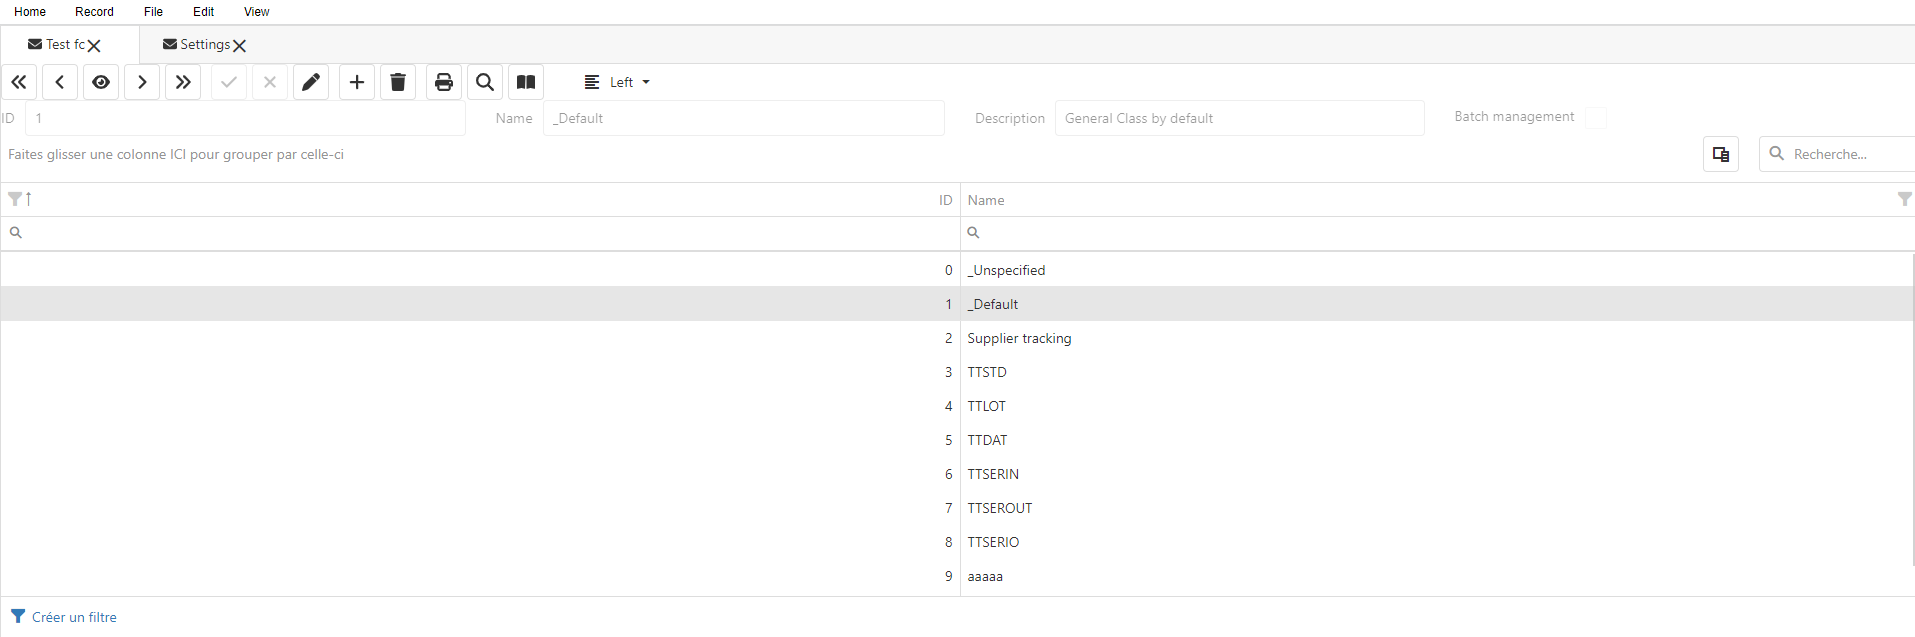
\includegraphics[width=0.7\linewidth]{images/mph_web_reactts_1.png}
					\end{center}
					\caption{Capture d'écran de l'application web morpheus}
					\label{fig:mph_web1}
				\end{figure}

				\begin{figure}[h!]
					\begin{center}
						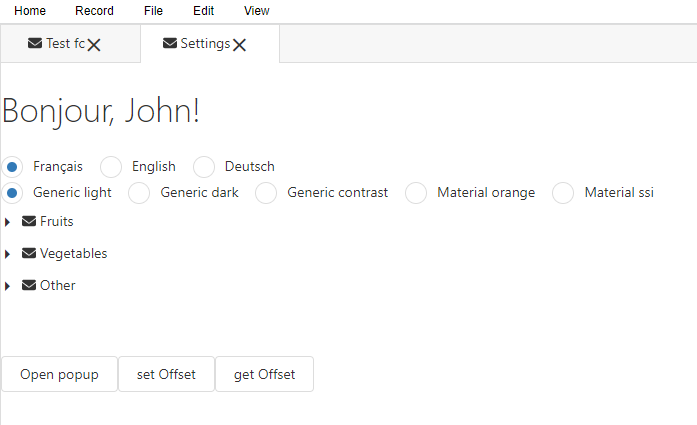
\includegraphics[width=0.7\linewidth]{images/mph_web_reactts_2.png}
					\end{center}
					\caption{Capture d'écran de l'application web morpheus}
					\label{fig:mph_web2}
				\end{figure}
				
			%\subsection{Résultats quantitatifs}
				%Utilisez cette sous-partie pour mettre en avant les résultats quantitatifs obtenus grâce à votre contribution au projet. Cela peut inclure des chiffres tels que des gains financiers, des augmentations de productivité, des réductions de coûts, etc.
			
				
			%\subsection{Résultats qualitatif}
				%Détaillez les résultats qualitatifs qui ont eu un impact positif sur l'entreprise. Cela peut inclure des améliorations de la qualité, de la satisfaction client, de la réputation de l'entreprise, etc.
			
			%\subsection{Comparaison avec les objectifs initiaux}
				%Comparez les réalisations et les résultats obtenus avec les objectifs initialement définis pour le projet. Mettez en évidence les écarts et expliquez comment ils ont été comblés.
				
			%\subsection{Réactions des parties prenantes}
				%Si possible, partagez des commentaires ou des réactions des parties prenantes du projet (par exemple, les clients, les supérieurs hiérarchiques, les collègues). Montrez comment votre travail a été perçu positivement.
				
			%\subsection{Mesure de l'impact global}
				%Analysez comment ces réalisations et résultats ont eu un impact global sur l'entreprise ou l'organisation. Expliquez comment ils ont contribué à atteindre des objectifs stratégiques plus larges.
				
			%\subsection{Leçons apprises}
				%Partagez les enseignements que vous avez tirés des réalisations et résultats du projet. Qu'avez-vous appris de cette expérience qui pourrait être appliqué à de futurs projets ?
			
			\subsection{Conclusion des réalisations et résultats}
				%Terminez en faisant une synthèse des réalisations clés et des résultats obtenus grâce à votre contribution au projet. Réfléchissez sur leur importance pour l'entreprise et sur la manière dont ils ont renforcé votre propre développement professionnel.
			
			\subsection{Conclusion du projet}
				%Présentez la conclusion du projet, y compris la réalisation de ses objectifs initiaux. Faites un bilan des résultats globaux et de l'impact sur l'entreprise.
			
			%Chacune de ces sous-parties contribue à donner une vue d'ensemble complète des réalisations et des résultats obtenus grâce à votre travail sur le projet. Veillez à maintenir une structure logique pour faciliter la compréhension de l'impact de vos actions.

		\newpage

		\section{Compétences mises en oeuvre}
			Chaque expérience professionnelle, notamment un stage, est une opportunité précieuse pour développer et mettre en œuvre des compétences essentielles. Au cours de mon stage au sein de SSI SCHÄFER, j'ai eu la chance de participer activement à un projet qui m'a permis d'acquérir et de mettre en œuvre diverses compétences professionnelles de manière concrète. Cette section est dédiée à ces compétences, qui sont le socle de ma croissance en tant que professionnel.\\

			Lorsque nous évoluons dans un environnement professionnel, il est essentiel de savoir identifier, adapter et appliquer nos compétences en réponse aux défis spécifiques rencontrés. Ce projet a été le terrain d'entraînement idéal pour mettre en pratique mes compétences, tout en les renforçant et en les perfectionnant. En partageant ces compétences mises en œuvre, je souhaite démontrer comment mon stage a été bien plus qu'une simple expérience d'observation, mais une réelle occasion d'apprentissage et de croissance professionnelle.\\

			Au fil de cette section, je vais mettre en avant les compétences clés que j'ai mobilisées et développées tout au long du projet, expliquer comment elles ont été appliquées dans un contexte professionnel concret, et montrer en quoi elles ont contribué aux réalisations et au succès du projet. Ces compétences, acquises au cours de mon stage, seront sans aucun doute un atout précieux dans ma future carrière professionnelle, et je suis enthousiaste à l'idée de les développer davantage dans des contextes similaires.

			\subsection{Compétences techniques}
				%Dans cette sous-partie, listez et détaillez les compétences techniques spécifiques que vous avez utilisées et développées pendant le projet. Cela peut inclure des compétences liées à la programmation, à l'analyse de données, à la gestion de projet, à l'utilisation d'outils spécifiques, etc.
				%Voici la liste des compétences techniques que j'ai pu développer au cours de mon stage.
				Les compétences techniques jouent un rôle central dans notre capacité à concevoir, développer, mettre en œuvre et optimiser l'application web morpheus. Tout au long de cette partie, nous allons mettre en lumière les compétences spécifiques que nous avons utilisées pour atteindre nos objectifs, en expliquant comment elles ont été appliquées dans un contexte professionnel.
				
				\subsubsection{Delphi}
				
				\subsubsection{HTML}
				
				\subsubsection{CSS}
				
				\subsubsection{Javascript}
				
				\subsubsection{ReactJS}
				
				\subsubsection{SQL}
				
				\subsubsection{Latex}
				
				\subsubsection{}
				\subsubsection{}
			
			
			\subsection{Compétences en gestion}
				%Expliquez comment vous avez appliqué des compétences en gestion tout au long du projet. Cela peut inclure la gestion du temps, la planification, la budgétisation, la gestion des ressources humaines, la résolution de problèmes, etc.
				La réussite de tout projet ou mission professionnelle repose non seulement sur des compétences techniques solides, mais également sur une expertise en gestion efficace. Dans cette section, nous explorerons les compétences en gestion que nous avons mises en œuvre tout au long de notre mission/stage/projet [nom de la mission/stage/projet] et comment elles ont contribué à la réalisation de nos objectifs.

Les compétences en gestion englobent un large éventail de capacités, notamment la planification stratégique, l'organisation, la gestion des ressources, la prise de décision, la communication, et la résolution de problèmes. Tout au long de cette partie, nous allons examiner comment nous avons appliqué ces compétences de manière spécifique et contextualisée dans notre mission/stage/projet.
				
				\subsubsection{Gestion du temps}

				\subsubsection{Planification}
			
			\subsection{Compétences en communication}
				%Mettez en avant vos compétences en communication, notamment comment vous avez interagi avec l'équipe du projet, les parties prenantes, les clients, et comment vous avez rédigé des rapports ou des documents techniques.
				La communication efficace est le cœur de toute entreprise ou projet réussi. Dans cette section, nous allons explorer en détail les compétences en communication que nous avons utilisées et développées tout au long de notre mission/stage/projet [nom de la mission/stage/projet] et comment elles ont été essentielles pour atteindre nos objectifs.
				
				\subsubsection{Rédaction d'une documentation technique}			


			%\subsection{Compétences en résolution de problèmes}
				%Détaillez comment vous avez utilisé vos compétences en résolution de problèmes pour aborder les défis qui se sont présentés au cours du projet. Présentez des exemples concrets de problèmes que vous avez résolus avec succès.
			
			%\subsection{Compétences en leadership}
				%Expliquez comment vous avez fait preuve de compétences en leadership, que ce soit en prenant des initiatives, en motivant l'équipe, en prenant des responsabilités ou en influençant positivement le projet.
				%\subsubsection{Choix du changement de langage de programmation}
			
			\subsection{Compétences en adaptabilité}
				%Mettez en évidence votre capacité à vous adapter à des situations changeantes ou imprévues au cours du projet. Montrez comment vous avez géré des scénarios imprévus avec succès.
				L'adaptabilité est une compétence clé dans le monde professionnel en rapide évolution d'aujourd'hui. Dans cette section, nous allons explorer comment notre capacité à nous adapter aux changements, aux défis et aux nouvelles situations a été mise en évidence tout au long de notre mission/stage/projet [nom de la mission/stage/projet] et comment cela a contribué à notre réussite.
				
				\subsubsection{Choix du changement de langage de programmation}
			
			\subsection{Compétences en analyse}
				%Présentez comment vous avez utilisé des compétences en analyse pour évaluer des données, des performances, des résultats, ou pour prendre des décisions basées sur des informations.
						
			%\subsection{Compétences en gestion du stress}
				%Si pertinent, partagez comment vous avez géré le stress ou la pression au cours du projet, et comment cela a contribué à la réussite globale.
			
			\subsection{Leçons apprises et développement professionnel}
				%Terminez en réfléchissant sur les compétences que vous avez développées tout au long du projet, sur leur importance pour votre développement professionnel, et sur la manière dont vous prévoyez de les utiliser dans l'avenir.
			
			%Chacune de ces sous-parties contribue à mettre en évidence les compétences spécifiques que vous avez développées et mises en œuvre pendant le projet. Veillez à illustrer vos compétences à l'aide d'exemples concrets et pertinents pour démontrer leur application dans un contexte professionnel.	
			
	
	\section{Conclusion}

	\newpage
	
	\phantomsection

	%\renewcommand{\bibname}{Bibliographie}
	%\addto{\captionsfrench}{\renewcommand{\bibname}{Bibliographie}}
	\renewcommand\refname{Bibliographie}
	%site internet morpheus à changer dire que les pages ne sont plus d'actualités...
	\bibliography{testbib}
	\bibliographystyle{ieeetr}%ieeetr %unsrt
	\addcontentsline{toc}{section}{Bibliographie}
	%\addcontentsline{toc}{section}{\bibliographyname}

	%\newpage

	\phantomsection
	\printindex

	\newpage

	\phantomsection
	\appendix
	\section*{Annexes}
	\addcontentsline{toc}{section}{Annexes}
		%si moins de 26 annexes
		\renewcommand{\thesubsection}{\Alph{subsection}}
		\counterwithin{figure}{subsection}
		\counterwithin{table}{subsection}
		%sinon
		%\renewcommand{\thesubsection}{\Roman{subsection}}

		\subsection{Dates importantes de l'histoire SSI SCHÄFER}\label{appendix:history}
			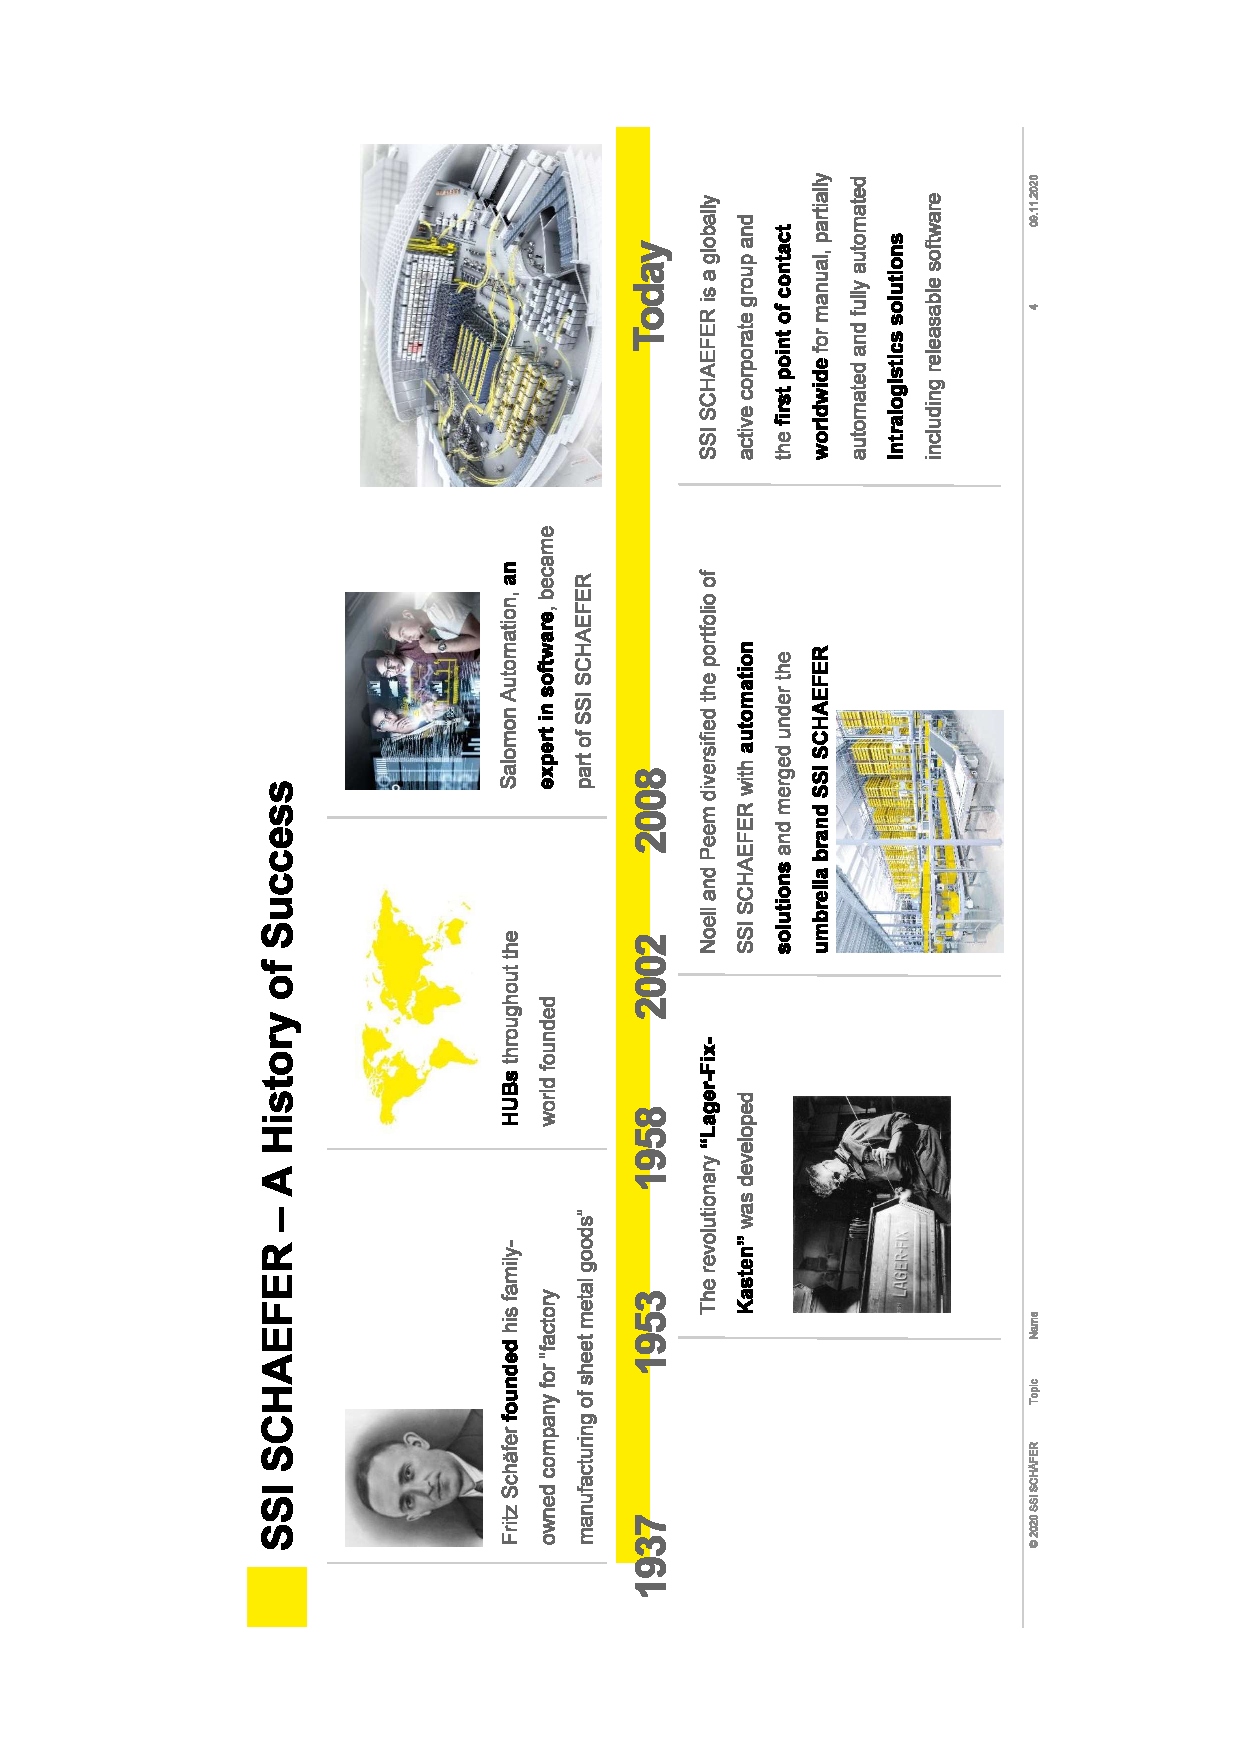
\includegraphics[width=0.8\linewidth]{images/history.pdf}

		\newpage
		\subsection{Carte des filiales SSI SCHÄFER}\label{appendix:map}
			\begin{center}
				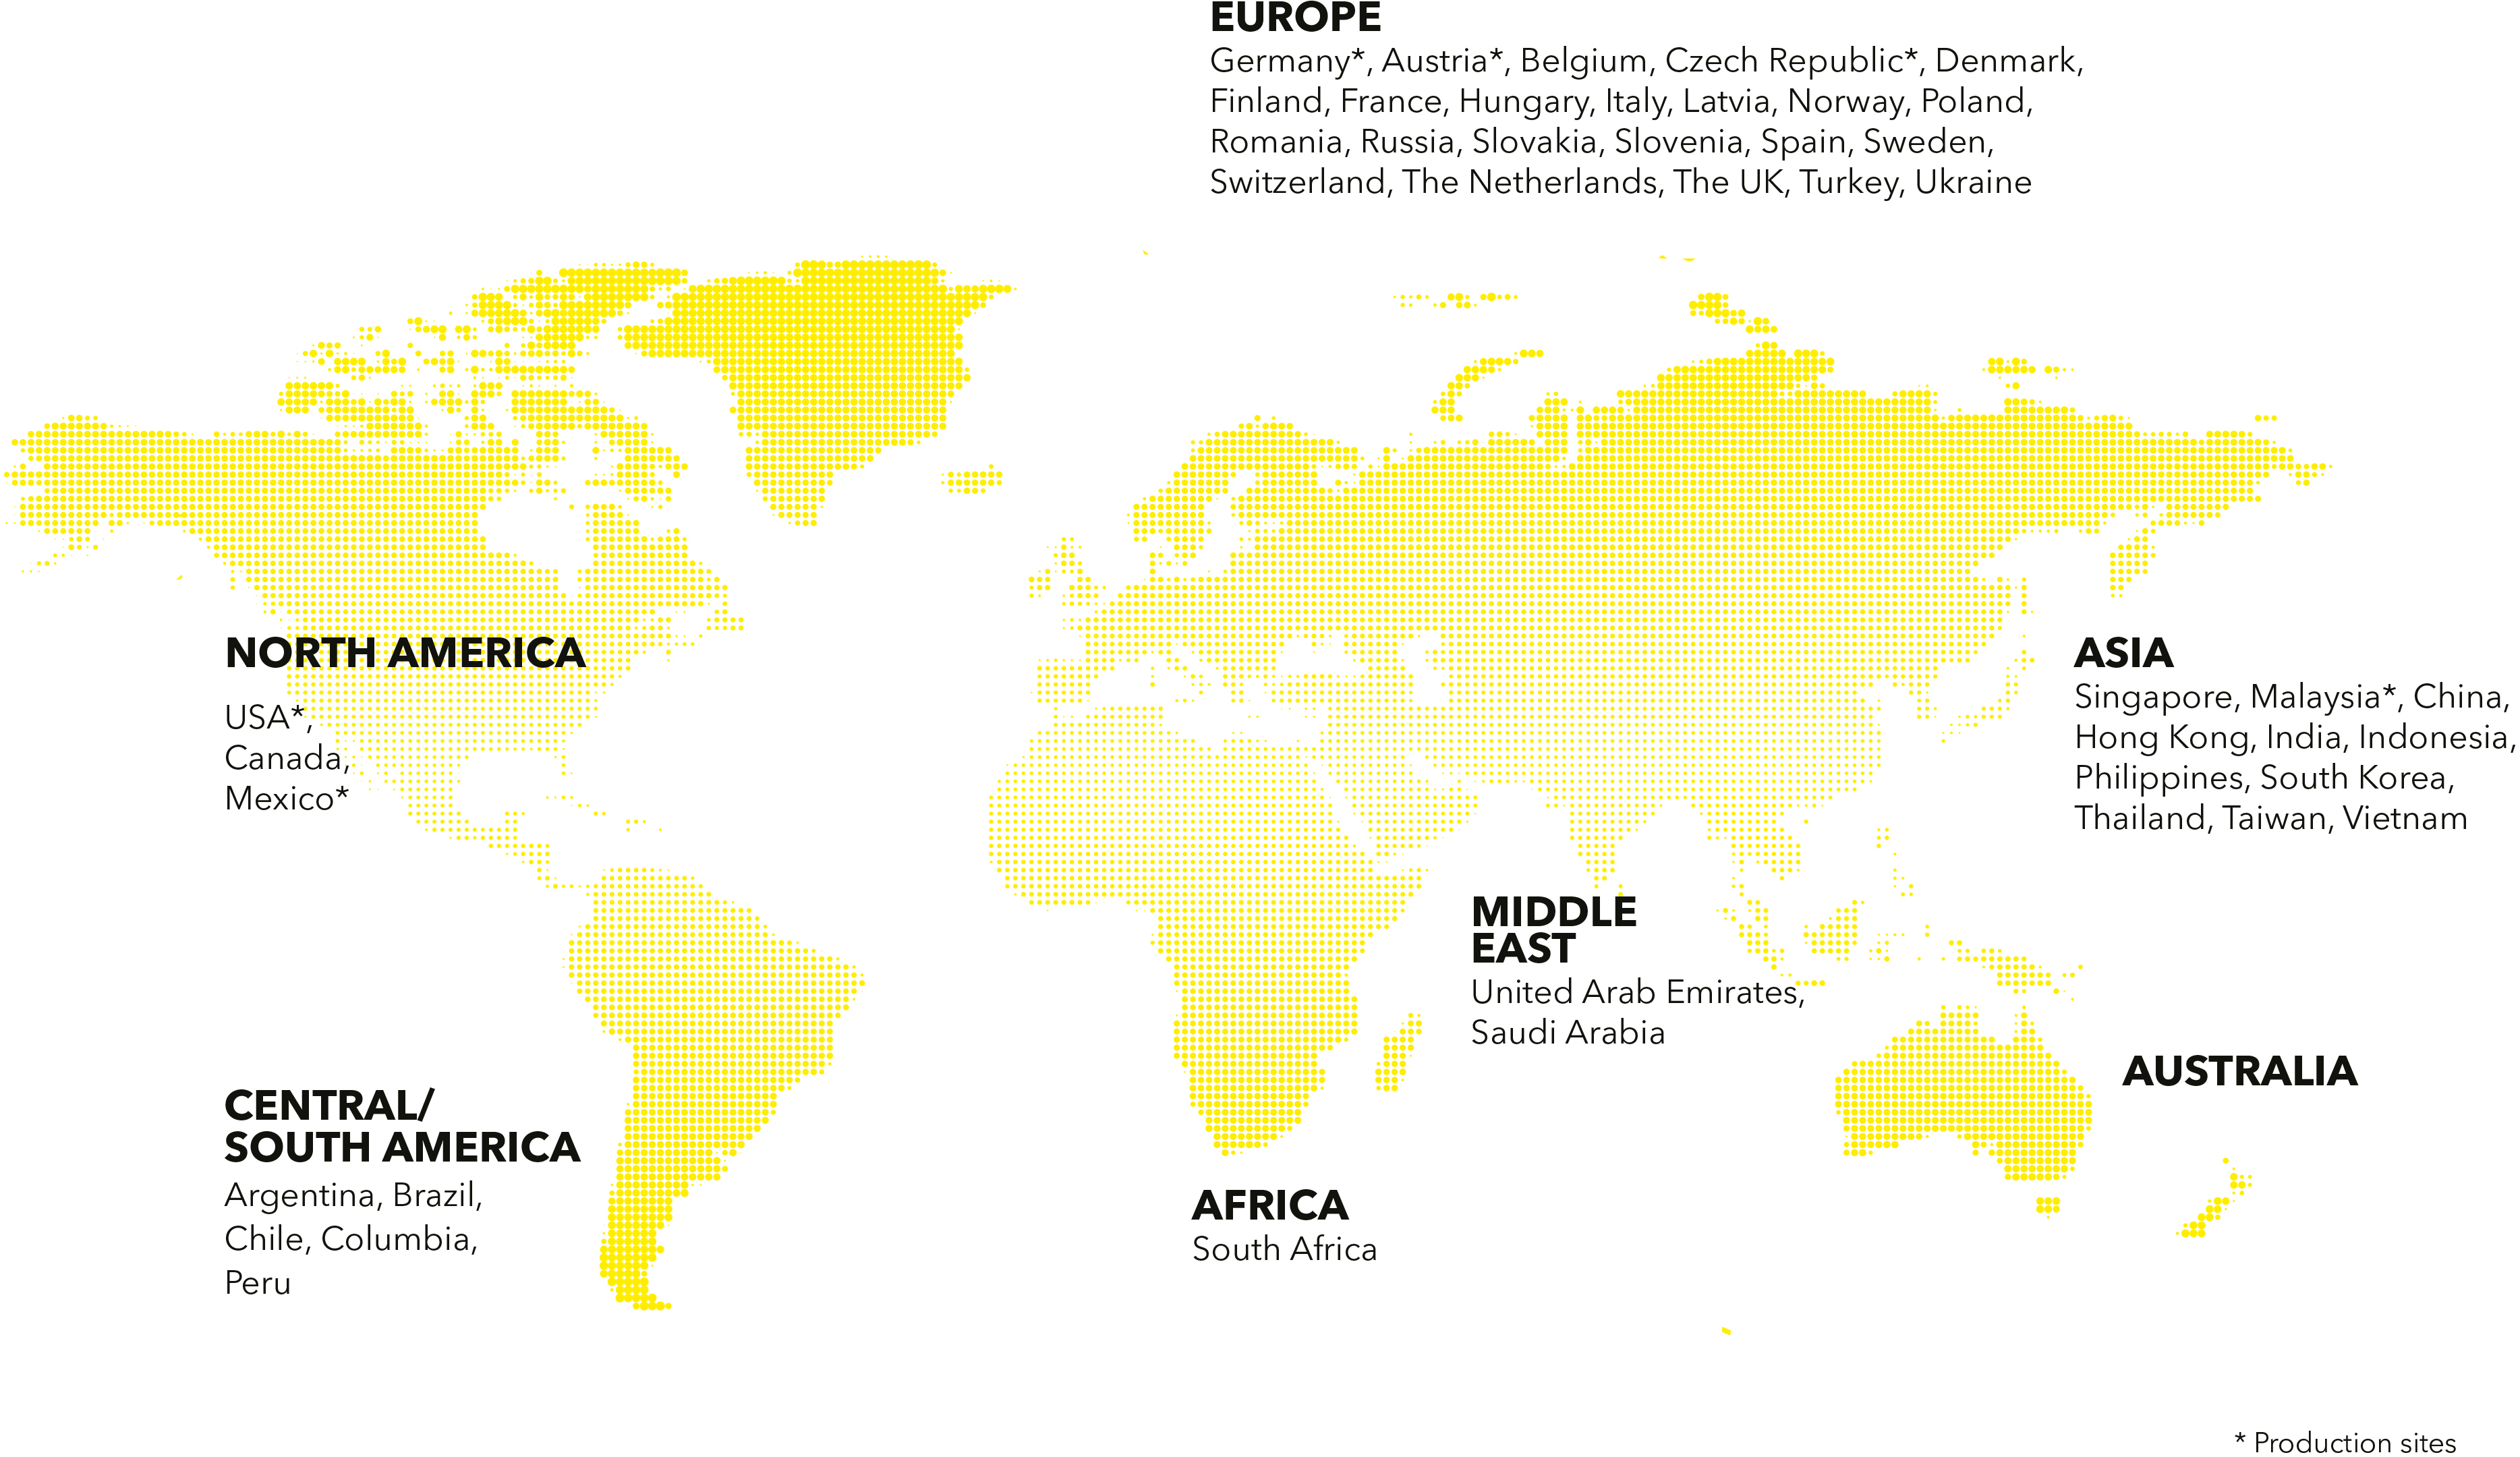
\includegraphics[width=\textwidth]{images/world_map.jpg}
			\end{center}
		\newpage


		\subsection{Liste complète des fonctionnalités de MORPHEUS WMS}\label{appendix:morpheusWMSFonctionnalites}
			\begin{figure}[h!]
					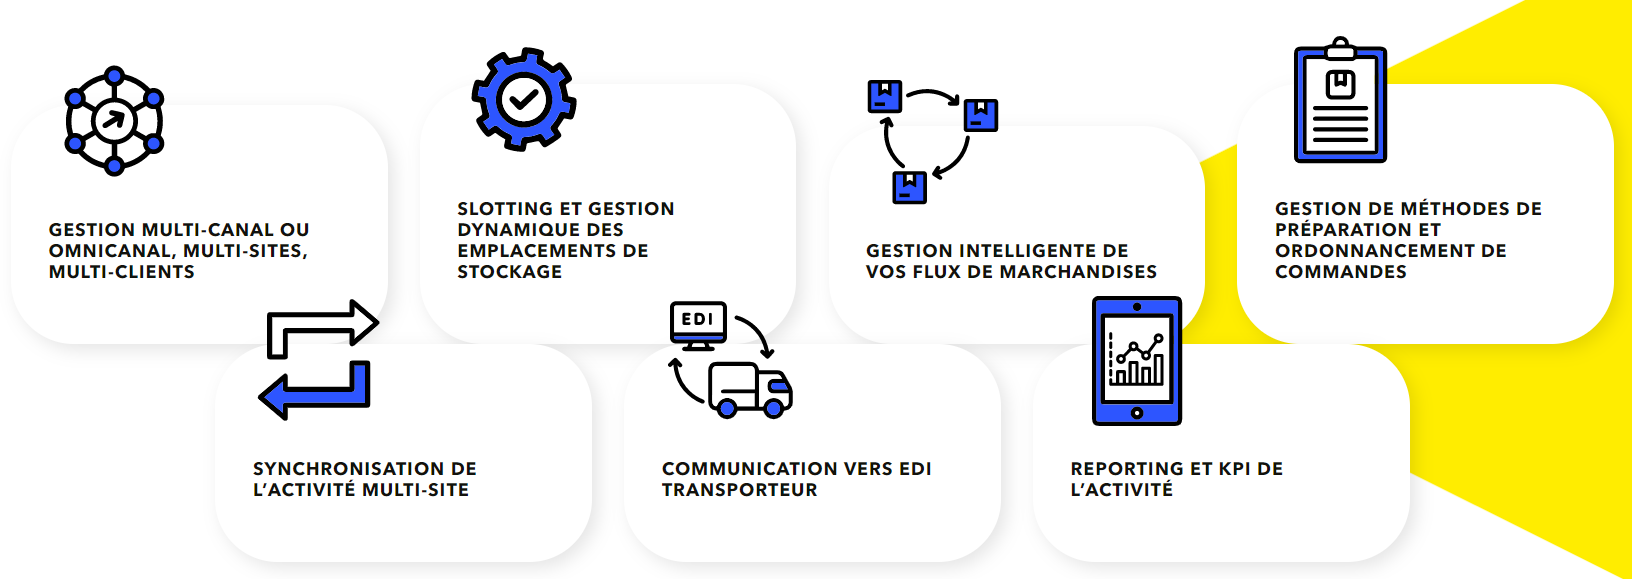
\includegraphics[width=\linewidth]{images/morpheus_wms_fonctionnalites.png}
					\caption{Fonctionnalités de Morpheus WMS}%\cite{screenshot}
					\label{fig:morpheus_wms_fonctionnalites}
			\end{figure}
		\subsection{Liste complète des fonctionnalités de MORPHEUS WCS}\label{appendix:morpheusWCSFonctionnalites}
			\begin{figure}[h!]
					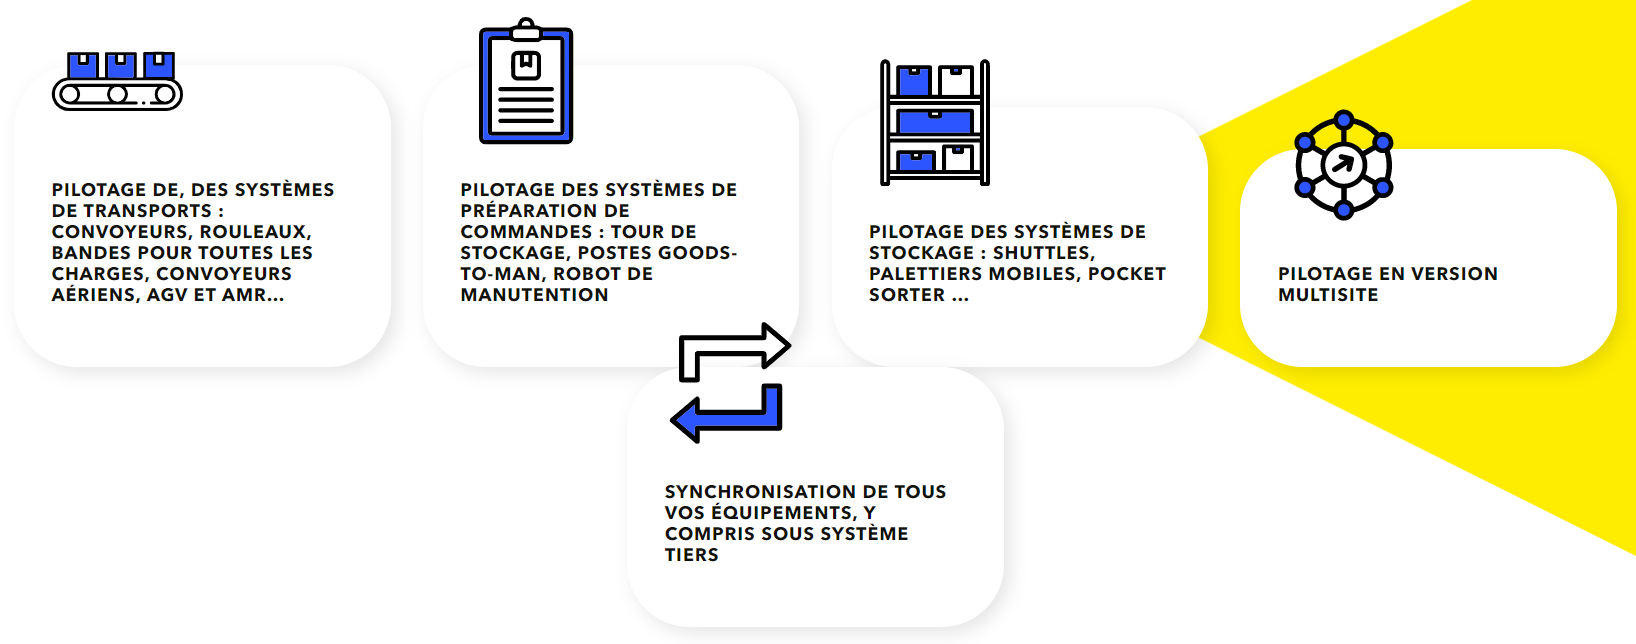
\includegraphics[width=\linewidth]{images/morpheus_wcs_fonctionnalites.png}
					\caption{Fonctionnalités de Morpheus WCS}%\cite{screenshot}
					\label{fig:morpheus_wcs_fonctionnalites}
			\end{figure}

		\newpage

	\section*{Mots clés}
	Liste des mots clés : delphi, développement, développement informatique, logistique, France, Cholet, WMS, WCS, MORPHEUS, tms, react, nodejs, devexpress, devextreme
	%en anglais
	%en allemand
	\newpage

	\phantomsection
	\section*{Résumés}
	\addcontentsline{toc}{section}{Résumés}
		\subsection*{Résumé}
		\addcontentsline{toc}{subsection}{Résumé}

		\subsection*{Summary}
		\addcontentsline{toc}{subsection}{Summary}


		\subsection*{Zusammenfassung}
		\addcontentsline{toc}{subsection}{Zusammenfassung}


	
		\newpage
\end{document}